% Created by tikzDevice version 0.6.2-92-0ad2792 on 2013-03-12 19:41:36
% !TEX encoding = UTF-8 Unicode
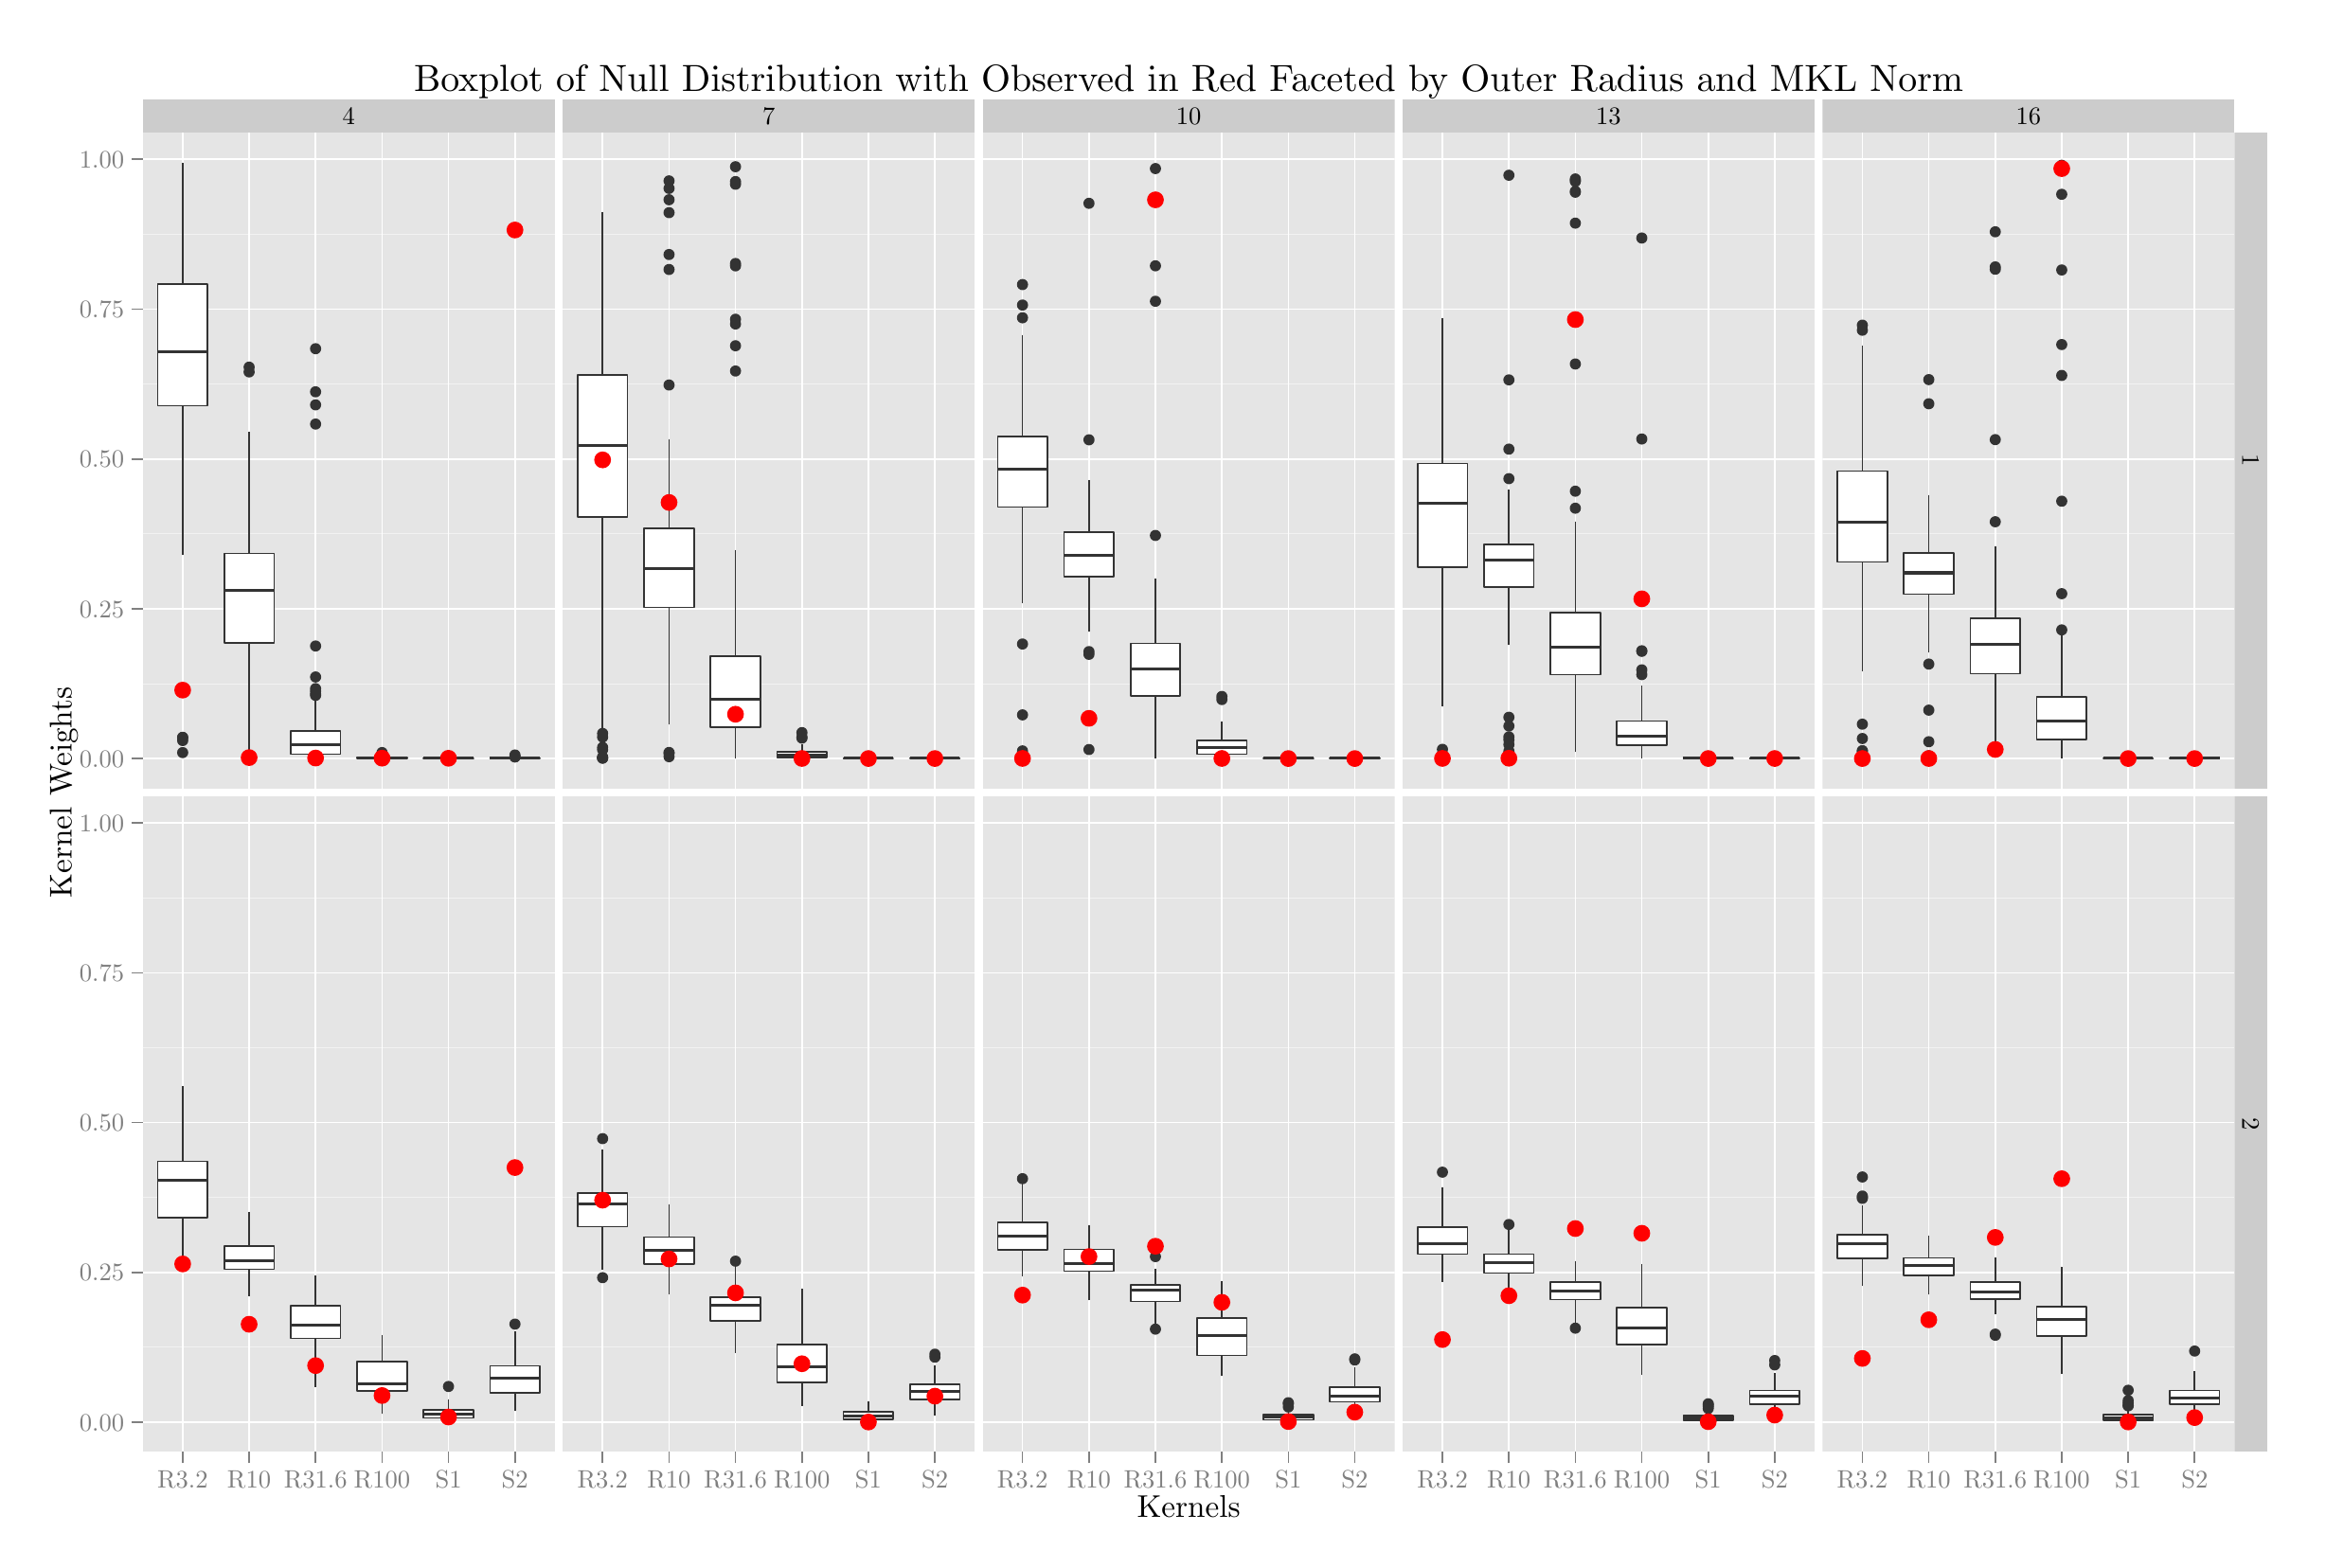
\begin{tikzpicture}[x=1pt,y=1pt]
\definecolor[named]{fillColor}{rgb}{1.00,1.00,1.00}
\path[use as bounding box,fill=fillColor,fill opacity=0.00] (0,0) rectangle (867.24,578.16);
\begin{scope}
\path[clip] (  0.00,  0.00) rectangle (867.24,578.16);
\definecolor[named]{drawColor}{rgb}{1.00,1.00,1.00}
\definecolor[named]{fillColor}{rgb}{1.00,1.00,1.00}

\path[draw=drawColor,line width= 0.6pt,line join=round,line cap=round,fill=fillColor] ( -0.00,  0.00) rectangle (867.24,578.16);
\end{scope}
\begin{scope}
\path[clip] ( 44.49,537.54) rectangle (201.69,550.17);
\definecolor[named]{fillColor}{rgb}{0.80,0.80,0.80}

\path[fill=fillColor] ( 44.49,537.54) rectangle (201.69,550.17);
\definecolor[named]{drawColor}{rgb}{0.00,0.00,0.00}

\node[text=drawColor,anchor=base,inner sep=0pt, outer sep=0pt, scale=  0.96] at (123.09,540.55) {4};
\end{scope}
\begin{scope}
\path[clip] (204.70,537.54) rectangle (361.91,550.17);
\definecolor[named]{fillColor}{rgb}{0.80,0.80,0.80}

\path[fill=fillColor] (204.70,537.54) rectangle (361.91,550.17);
\definecolor[named]{drawColor}{rgb}{0.00,0.00,0.00}

\node[text=drawColor,anchor=base,inner sep=0pt, outer sep=0pt, scale=  0.96] at (283.31,540.55) {7};
\end{scope}
\begin{scope}
\path[clip] (364.92,537.54) rectangle (522.13,550.17);
\definecolor[named]{fillColor}{rgb}{0.80,0.80,0.80}

\path[fill=fillColor] (364.92,537.54) rectangle (522.13,550.17);
\definecolor[named]{drawColor}{rgb}{0.00,0.00,0.00}

\node[text=drawColor,anchor=base,inner sep=0pt, outer sep=0pt, scale=  0.96] at (443.52,540.55) {10};
\end{scope}
\begin{scope}
\path[clip] (525.14,537.54) rectangle (682.34,550.17);
\definecolor[named]{fillColor}{rgb}{0.80,0.80,0.80}

\path[fill=fillColor] (525.14,537.54) rectangle (682.34,550.17);
\definecolor[named]{drawColor}{rgb}{0.00,0.00,0.00}

\node[text=drawColor,anchor=base,inner sep=0pt, outer sep=0pt, scale=  0.96] at (603.74,540.55) {13};
\end{scope}
\begin{scope}
\path[clip] (685.35,537.54) rectangle (842.56,550.17);
\definecolor[named]{fillColor}{rgb}{0.80,0.80,0.80}

\path[fill=fillColor] (685.35,537.54) rectangle (842.56,550.17);
\definecolor[named]{drawColor}{rgb}{0.00,0.00,0.00}

\node[text=drawColor,anchor=base,inner sep=0pt, outer sep=0pt, scale=  0.96] at (763.96,540.55) {16};
\end{scope}
\begin{scope}
\path[clip] ( 44.49,287.29) rectangle (201.69,537.54);
\definecolor[named]{fillColor}{rgb}{0.90,0.90,0.90}

\path[fill=fillColor] ( 44.49,287.29) rectangle (201.69,537.54);
\definecolor[named]{drawColor}{rgb}{0.95,0.95,0.95}

\path[draw=drawColor,line width= 0.3pt,line join=round] ( 44.49,327.25) --
	(201.69,327.25);

\path[draw=drawColor,line width= 0.3pt,line join=round] ( 44.49,384.42) --
	(201.69,384.42);

\path[draw=drawColor,line width= 0.3pt,line join=round] ( 44.49,441.60) --
	(201.69,441.60);

\path[draw=drawColor,line width= 0.3pt,line join=round] ( 44.49,498.77) --
	(201.69,498.77);
\definecolor[named]{drawColor}{rgb}{1.00,1.00,1.00}

\path[draw=drawColor,line width= 0.6pt,line join=round] ( 44.49,298.67) --
	(201.69,298.67);

\path[draw=drawColor,line width= 0.6pt,line join=round] ( 44.49,355.84) --
	(201.69,355.84);

\path[draw=drawColor,line width= 0.6pt,line join=round] ( 44.49,413.01) --
	(201.69,413.01);

\path[draw=drawColor,line width= 0.6pt,line join=round] ( 44.49,470.18) --
	(201.69,470.18);

\path[draw=drawColor,line width= 0.6pt,line join=round] ( 44.49,527.35) --
	(201.69,527.35);

\path[draw=drawColor,line width= 0.6pt,line join=round] ( 59.70,287.29) --
	( 59.70,537.54);

\path[draw=drawColor,line width= 0.6pt,line join=round] ( 85.05,287.29) --
	( 85.05,537.54);

\path[draw=drawColor,line width= 0.6pt,line join=round] (110.41,287.29) --
	(110.41,537.54);

\path[draw=drawColor,line width= 0.6pt,line join=round] (135.77,287.29) --
	(135.77,537.54);

\path[draw=drawColor,line width= 0.6pt,line join=round] (161.12,287.29) --
	(161.12,537.54);

\path[draw=drawColor,line width= 0.6pt,line join=round] (186.48,287.29) --
	(186.48,537.54);
\definecolor[named]{fillColor}{rgb}{0.20,0.20,0.20}

\path[fill=fillColor] ( 59.70,306.66) circle (  2.13);

\path[fill=fillColor] ( 59.70,306.78) circle (  2.13);

\path[fill=fillColor] ( 59.70,305.54) circle (  2.13);

\path[fill=fillColor] ( 59.70,300.94) circle (  2.13);
\definecolor[named]{drawColor}{rgb}{0.20,0.20,0.20}

\path[draw=drawColor,line width= 0.6pt,line join=round,fill=fillColor] ( 59.70,479.74) -- ( 59.70,526.17);

\path[draw=drawColor,line width= 0.6pt,line join=round,fill=fillColor] ( 59.70,433.37) -- ( 59.70,376.41);
\definecolor[named]{fillColor}{rgb}{1.00,1.00,1.00}

\path[draw=drawColor,line width= 0.6pt,line join=round,line cap=round,fill=fillColor] ( 50.19,479.74) --
	( 50.19,433.37) --
	( 69.21,433.37) --
	( 69.21,479.74) --
	( 50.19,479.74) --
	cycle;
\definecolor[named]{fillColor}{rgb}{0.20,0.20,0.20}

\path[draw=drawColor,line width= 1.1pt,line join=round,fill=fillColor] ( 50.19,454.02) -- ( 69.21,454.02);

\path[fill=fillColor] ( 85.05,448.04) circle (  2.13);

\path[fill=fillColor] ( 85.05,446.21) circle (  2.13);

\path[draw=drawColor,line width= 0.6pt,line join=round,fill=fillColor] ( 85.05,376.92) -- ( 85.05,423.44);

\path[draw=drawColor,line width= 0.6pt,line join=round,fill=fillColor] ( 85.05,342.68) -- ( 85.05,299.83);
\definecolor[named]{fillColor}{rgb}{1.00,1.00,1.00}

\path[draw=drawColor,line width= 0.6pt,line join=round,line cap=round,fill=fillColor] ( 75.55,376.92) --
	( 75.55,342.68) --
	( 94.56,342.68) --
	( 94.56,376.92) --
	( 75.55,376.92) --
	cycle;
\definecolor[named]{fillColor}{rgb}{0.20,0.20,0.20}

\path[draw=drawColor,line width= 1.1pt,line join=round,fill=fillColor] ( 75.55,362.69) -- ( 94.56,362.69);

\path[fill=fillColor] (110.41,341.62) circle (  2.13);

\path[fill=fillColor] (110.41,324.34) circle (  2.13);

\path[fill=fillColor] (110.41,329.80) circle (  2.13);

\path[fill=fillColor] (110.41,323.32) circle (  2.13);

\path[fill=fillColor] (110.41,325.35) circle (  2.13);

\path[fill=fillColor] (110.41,322.77) circle (  2.13);

\path[fill=fillColor] (110.41,426.32) circle (  2.13);

\path[fill=fillColor] (110.41,438.63) circle (  2.13);

\path[fill=fillColor] (110.41,433.65) circle (  2.13);

\path[fill=fillColor] (110.41,455.08) circle (  2.13);

\path[draw=drawColor,line width= 0.6pt,line join=round,fill=fillColor] (110.41,309.13) -- (110.41,322.21);

\path[draw=drawColor,line width= 0.6pt,line join=round,fill=fillColor] (110.41,300.39) -- (110.41,298.68);
\definecolor[named]{fillColor}{rgb}{1.00,1.00,1.00}

\path[draw=drawColor,line width= 0.6pt,line join=round,line cap=round,fill=fillColor] (100.90,309.13) --
	(100.90,300.39) --
	(119.92,300.39) --
	(119.92,309.13) --
	(100.90,309.13) --
	cycle;
\definecolor[named]{fillColor}{rgb}{0.20,0.20,0.20}

\path[draw=drawColor,line width= 1.1pt,line join=round,fill=fillColor] (100.90,303.91) -- (119.92,303.91);

\path[fill=fillColor] (135.77,299.88) circle (  2.13);

\path[fill=fillColor] (135.77,300.96) circle (  2.13);

\path[fill=fillColor] (135.77,299.58) circle (  2.13);

\path[fill=fillColor] (135.77,299.61) circle (  2.13);

\path[fill=fillColor] (135.77,299.80) circle (  2.13);

\path[fill=fillColor] (135.77,299.66) circle (  2.13);

\path[fill=fillColor] (135.77,299.60) circle (  2.13);

\path[draw=drawColor,line width= 0.6pt,line join=round,fill=fillColor] (135.77,299.10) -- (135.77,299.55);

\path[draw=drawColor,line width= 0.6pt,line join=round,fill=fillColor] (135.77,298.78) -- (135.77,298.67);
\definecolor[named]{fillColor}{rgb}{1.00,1.00,1.00}

\path[draw=drawColor,line width= 0.6pt,line join=round,line cap=round,fill=fillColor] (126.26,299.10) --
	(126.26,298.78) --
	(145.27,298.78) --
	(145.27,299.10) --
	(126.26,299.10) --
	cycle;
\definecolor[named]{fillColor}{rgb}{0.20,0.20,0.20}

\path[draw=drawColor,line width= 1.1pt,line join=round,fill=fillColor] (126.26,298.92) -- (145.27,298.92);

\path[draw=drawColor,line width= 0.6pt,line join=round,fill=fillColor] (161.12,298.83) -- (161.12,298.99);

\path[draw=drawColor,line width= 0.6pt,line join=round,fill=fillColor] (161.12,298.70) -- (161.12,298.67);
\definecolor[named]{fillColor}{rgb}{1.00,1.00,1.00}

\path[draw=drawColor,line width= 0.6pt,line join=round,line cap=round,fill=fillColor] (151.61,298.83) --
	(151.61,298.70) --
	(170.63,298.70) --
	(170.63,298.83) --
	(151.61,298.83) --
	cycle;
\definecolor[named]{fillColor}{rgb}{0.20,0.20,0.20}

\path[draw=drawColor,line width= 1.1pt,line join=round,fill=fillColor] (151.61,298.76) -- (170.63,298.76);

\path[fill=fillColor] (186.48,300.03) circle (  2.13);

\path[fill=fillColor] (186.48,299.32) circle (  2.13);

\path[fill=fillColor] (186.48,299.29) circle (  2.13);

\path[draw=drawColor,line width= 0.6pt,line join=round,fill=fillColor] (186.48,298.92) -- (186.48,299.20);

\path[draw=drawColor,line width= 0.6pt,line join=round,fill=fillColor] (186.48,298.71) -- (186.48,298.67);
\definecolor[named]{fillColor}{rgb}{1.00,1.00,1.00}

\path[draw=drawColor,line width= 0.6pt,line join=round,line cap=round,fill=fillColor] (176.97,298.92) --
	(176.97,298.71) --
	(195.99,298.71) --
	(195.99,298.92) --
	(176.97,298.92) --
	cycle;
\definecolor[named]{fillColor}{rgb}{0.20,0.20,0.20}

\path[draw=drawColor,line width= 1.1pt,line join=round,fill=fillColor] (176.97,298.83) -- (195.99,298.83);
\definecolor[named]{fillColor}{rgb}{1.00,0.00,0.00}

\path[fill=fillColor] ( 59.70,324.79) circle (  3.20);

\path[fill=fillColor] ( 85.05,299.04) circle (  3.20);

\path[fill=fillColor] (110.41,298.87) circle (  3.20);

\path[fill=fillColor] (135.77,298.82) circle (  3.20);

\path[fill=fillColor] (161.12,298.78) circle (  3.20);

\path[fill=fillColor] (186.48,500.38) circle (  3.20);
\end{scope}
\begin{scope}
\path[clip] ( 44.49, 34.03) rectangle (201.69,284.28);
\definecolor[named]{fillColor}{rgb}{0.90,0.90,0.90}

\path[fill=fillColor] ( 44.49, 34.03) rectangle (201.69,284.28);
\definecolor[named]{drawColor}{rgb}{0.95,0.95,0.95}

\path[draw=drawColor,line width= 0.3pt,line join=round] ( 44.49, 73.99) --
	(201.69, 73.99);

\path[draw=drawColor,line width= 0.3pt,line join=round] ( 44.49,131.17) --
	(201.69,131.17);

\path[draw=drawColor,line width= 0.3pt,line join=round] ( 44.49,188.34) --
	(201.69,188.34);

\path[draw=drawColor,line width= 0.3pt,line join=round] ( 44.49,245.51) --
	(201.69,245.51);
\definecolor[named]{drawColor}{rgb}{1.00,1.00,1.00}

\path[draw=drawColor,line width= 0.6pt,line join=round] ( 44.49, 45.41) --
	(201.69, 45.41);

\path[draw=drawColor,line width= 0.6pt,line join=round] ( 44.49,102.58) --
	(201.69,102.58);

\path[draw=drawColor,line width= 0.6pt,line join=round] ( 44.49,159.75) --
	(201.69,159.75);

\path[draw=drawColor,line width= 0.6pt,line join=round] ( 44.49,216.92) --
	(201.69,216.92);

\path[draw=drawColor,line width= 0.6pt,line join=round] ( 44.49,274.10) --
	(201.69,274.10);

\path[draw=drawColor,line width= 0.6pt,line join=round] ( 59.70, 34.03) --
	( 59.70,284.28);

\path[draw=drawColor,line width= 0.6pt,line join=round] ( 85.05, 34.03) --
	( 85.05,284.28);

\path[draw=drawColor,line width= 0.6pt,line join=round] (110.41, 34.03) --
	(110.41,284.28);

\path[draw=drawColor,line width= 0.6pt,line join=round] (135.77, 34.03) --
	(135.77,284.28);

\path[draw=drawColor,line width= 0.6pt,line join=round] (161.12, 34.03) --
	(161.12,284.28);

\path[draw=drawColor,line width= 0.6pt,line join=round] (186.48, 34.03) --
	(186.48,284.28);
\definecolor[named]{drawColor}{rgb}{0.20,0.20,0.20}
\definecolor[named]{fillColor}{rgb}{0.20,0.20,0.20}

\path[draw=drawColor,line width= 0.6pt,line join=round,fill=fillColor] ( 59.70,145.01) -- ( 59.70,173.63);

\path[draw=drawColor,line width= 0.6pt,line join=round,fill=fillColor] ( 59.70,123.45) -- ( 59.70,104.13);
\definecolor[named]{fillColor}{rgb}{1.00,1.00,1.00}

\path[draw=drawColor,line width= 0.6pt,line join=round,line cap=round,fill=fillColor] ( 50.19,145.01) --
	( 50.19,123.45) --
	( 69.21,123.45) --
	( 69.21,145.01) --
	( 50.19,145.01) --
	cycle;
\definecolor[named]{fillColor}{rgb}{0.20,0.20,0.20}

\path[draw=drawColor,line width= 1.1pt,line join=round,fill=fillColor] ( 50.19,137.68) -- ( 69.21,137.68);

\path[draw=drawColor,line width= 0.6pt,line join=round,fill=fillColor] ( 85.05,112.74) -- ( 85.05,125.63);

\path[draw=drawColor,line width= 0.6pt,line join=round,fill=fillColor] ( 85.05,103.81) -- ( 85.05, 93.37);
\definecolor[named]{fillColor}{rgb}{1.00,1.00,1.00}

\path[draw=drawColor,line width= 0.6pt,line join=round,line cap=round,fill=fillColor] ( 75.55,112.74) --
	( 75.55,103.81) --
	( 94.56,103.81) --
	( 94.56,112.74) --
	( 75.55,112.74) --
	cycle;
\definecolor[named]{fillColor}{rgb}{0.20,0.20,0.20}

\path[draw=drawColor,line width= 1.1pt,line join=round,fill=fillColor] ( 75.55,107.10) -- ( 94.56,107.10);

\path[draw=drawColor,line width= 0.6pt,line join=round,fill=fillColor] (110.41, 89.83) -- (110.41,101.25);

\path[draw=drawColor,line width= 0.6pt,line join=round,fill=fillColor] (110.41, 77.33) -- (110.41, 58.72);
\definecolor[named]{fillColor}{rgb}{1.00,1.00,1.00}

\path[draw=drawColor,line width= 0.6pt,line join=round,line cap=round,fill=fillColor] (100.90, 89.83) --
	(100.90, 77.33) --
	(119.92, 77.33) --
	(119.92, 89.83) --
	(100.90, 89.83) --
	cycle;
\definecolor[named]{fillColor}{rgb}{0.20,0.20,0.20}

\path[draw=drawColor,line width= 1.1pt,line join=round,fill=fillColor] (100.90, 82.37) -- (119.92, 82.37);

\path[draw=drawColor,line width= 0.6pt,line join=round,fill=fillColor] (135.77, 68.44) -- (135.77, 78.68);

\path[draw=drawColor,line width= 0.6pt,line join=round,fill=fillColor] (135.77, 57.31) -- (135.77, 48.67);
\definecolor[named]{fillColor}{rgb}{1.00,1.00,1.00}

\path[draw=drawColor,line width= 0.6pt,line join=round,line cap=round,fill=fillColor] (126.26, 68.44) --
	(126.26, 57.31) --
	(145.27, 57.31) --
	(145.27, 68.44) --
	(126.26, 68.44) --
	cycle;
\definecolor[named]{fillColor}{rgb}{0.20,0.20,0.20}

\path[draw=drawColor,line width= 1.1pt,line join=round,fill=fillColor] (126.26, 59.96) -- (145.27, 59.96);

\path[fill=fillColor] (161.12, 59.04) circle (  2.13);

\path[draw=drawColor,line width= 0.6pt,line join=round,fill=fillColor] (161.12, 50.06) -- (161.12, 54.26);

\path[draw=drawColor,line width= 0.6pt,line join=round,fill=fillColor] (161.12, 47.03) -- (161.12, 45.65);
\definecolor[named]{fillColor}{rgb}{1.00,1.00,1.00}

\path[draw=drawColor,line width= 0.6pt,line join=round,line cap=round,fill=fillColor] (151.61, 50.06) --
	(151.61, 47.03) --
	(170.63, 47.03) --
	(170.63, 50.06) --
	(151.61, 50.06) --
	cycle;
\definecolor[named]{fillColor}{rgb}{0.20,0.20,0.20}

\path[draw=drawColor,line width= 1.1pt,line join=round,fill=fillColor] (151.61, 48.43) -- (170.63, 48.43);

\path[fill=fillColor] (186.48, 82.84) circle (  2.13);

\path[draw=drawColor,line width= 0.6pt,line join=round,fill=fillColor] (186.48, 66.90) -- (186.48, 80.27);

\path[draw=drawColor,line width= 0.6pt,line join=round,fill=fillColor] (186.48, 56.66) -- (186.48, 49.59);
\definecolor[named]{fillColor}{rgb}{1.00,1.00,1.00}

\path[draw=drawColor,line width= 0.6pt,line join=round,line cap=round,fill=fillColor] (176.97, 66.90) --
	(176.97, 56.66) --
	(195.99, 56.66) --
	(195.99, 66.90) --
	(176.97, 66.90) --
	cycle;
\definecolor[named]{fillColor}{rgb}{0.20,0.20,0.20}

\path[draw=drawColor,line width= 1.1pt,line join=round,fill=fillColor] (176.97, 62.30) -- (195.99, 62.30);
\definecolor[named]{fillColor}{rgb}{1.00,0.00,0.00}

\path[fill=fillColor] ( 59.70,105.80) circle (  3.20);

\path[fill=fillColor] ( 85.05, 82.78) circle (  3.20);

\path[fill=fillColor] (110.41, 67.00) circle (  3.20);

\path[fill=fillColor] (135.77, 55.58) circle (  3.20);

\path[fill=fillColor] (161.12, 47.39) circle (  3.20);

\path[fill=fillColor] (186.48,142.58) circle (  3.20);
\end{scope}
\begin{scope}
\path[clip] (204.70,287.29) rectangle (361.91,537.54);
\definecolor[named]{fillColor}{rgb}{0.90,0.90,0.90}

\path[fill=fillColor] (204.70,287.29) rectangle (361.91,537.54);
\definecolor[named]{drawColor}{rgb}{0.95,0.95,0.95}

\path[draw=drawColor,line width= 0.3pt,line join=round] (204.70,327.25) --
	(361.91,327.25);

\path[draw=drawColor,line width= 0.3pt,line join=round] (204.70,384.42) --
	(361.91,384.42);

\path[draw=drawColor,line width= 0.3pt,line join=round] (204.70,441.60) --
	(361.91,441.60);

\path[draw=drawColor,line width= 0.3pt,line join=round] (204.70,498.77) --
	(361.91,498.77);
\definecolor[named]{drawColor}{rgb}{1.00,1.00,1.00}

\path[draw=drawColor,line width= 0.6pt,line join=round] (204.70,298.67) --
	(361.91,298.67);

\path[draw=drawColor,line width= 0.6pt,line join=round] (204.70,355.84) --
	(361.91,355.84);

\path[draw=drawColor,line width= 0.6pt,line join=round] (204.70,413.01) --
	(361.91,413.01);

\path[draw=drawColor,line width= 0.6pt,line join=round] (204.70,470.18) --
	(361.91,470.18);

\path[draw=drawColor,line width= 0.6pt,line join=round] (204.70,527.35) --
	(361.91,527.35);

\path[draw=drawColor,line width= 0.6pt,line join=round] (219.92,287.29) --
	(219.92,537.54);

\path[draw=drawColor,line width= 0.6pt,line join=round] (245.27,287.29) --
	(245.27,537.54);

\path[draw=drawColor,line width= 0.6pt,line join=round] (270.63,287.29) --
	(270.63,537.54);

\path[draw=drawColor,line width= 0.6pt,line join=round] (295.98,287.29) --
	(295.98,537.54);

\path[draw=drawColor,line width= 0.6pt,line join=round] (321.34,287.29) --
	(321.34,537.54);

\path[draw=drawColor,line width= 0.6pt,line join=round] (346.70,287.29) --
	(346.70,537.54);
\definecolor[named]{fillColor}{rgb}{0.20,0.20,0.20}

\path[fill=fillColor] (219.92,302.03) circle (  2.13);

\path[fill=fillColor] (219.92,298.86) circle (  2.13);

\path[fill=fillColor] (219.92,298.91) circle (  2.13);

\path[fill=fillColor] (219.92,306.85) circle (  2.13);

\path[fill=fillColor] (219.92,308.26) circle (  2.13);

\path[fill=fillColor] (219.92,302.95) circle (  2.13);

\path[fill=fillColor] (219.92,299.26) circle (  2.13);

\path[fill=fillColor] (219.92,298.83) circle (  2.13);
\definecolor[named]{drawColor}{rgb}{0.20,0.20,0.20}

\path[draw=drawColor,line width= 0.6pt,line join=round,fill=fillColor] (219.92,445.00) -- (219.92,507.06);

\path[draw=drawColor,line width= 0.6pt,line join=round,fill=fillColor] (219.92,390.83) -- (219.92,309.67);
\definecolor[named]{fillColor}{rgb}{1.00,1.00,1.00}

\path[draw=drawColor,line width= 0.6pt,line join=round,line cap=round,fill=fillColor] (210.41,445.00) --
	(210.41,390.83) --
	(229.42,390.83) --
	(229.42,445.00) --
	(210.41,445.00) --
	cycle;
\definecolor[named]{fillColor}{rgb}{0.20,0.20,0.20}

\path[draw=drawColor,line width= 1.1pt,line join=round,fill=fillColor] (210.41,418.25) -- (229.42,418.25);

\path[fill=fillColor] (245.27,441.23) circle (  2.13);

\path[fill=fillColor] (245.27,519.12) circle (  2.13);

\path[fill=fillColor] (245.27,491.02) circle (  2.13);

\path[fill=fillColor] (245.27,511.92) circle (  2.13);

\path[fill=fillColor] (245.27,485.31) circle (  2.13);

\path[fill=fillColor] (245.27,507.00) circle (  2.13);

\path[fill=fillColor] (245.27,301.00) circle (  2.13);

\path[fill=fillColor] (245.27,299.37) circle (  2.13);

\path[fill=fillColor] (245.27,516.25) circle (  2.13);

\path[fill=fillColor] (245.27,300.64) circle (  2.13);

\path[draw=drawColor,line width= 0.6pt,line join=round,fill=fillColor] (245.27,386.63) -- (245.27,420.47);

\path[draw=drawColor,line width= 0.6pt,line join=round,fill=fillColor] (245.27,356.31) -- (245.27,311.60);
\definecolor[named]{fillColor}{rgb}{1.00,1.00,1.00}

\path[draw=drawColor,line width= 0.6pt,line join=round,line cap=round,fill=fillColor] (235.76,386.63) --
	(235.76,356.31) --
	(254.78,356.31) --
	(254.78,386.63) --
	(235.76,386.63) --
	cycle;
\definecolor[named]{fillColor}{rgb}{0.20,0.20,0.20}

\path[draw=drawColor,line width= 1.1pt,line join=round,fill=fillColor] (235.76,371.27) -- (254.78,371.27);

\path[fill=fillColor] (270.63,486.69) circle (  2.13);

\path[fill=fillColor] (270.63,464.52) circle (  2.13);

\path[fill=fillColor] (270.63,466.33) circle (  2.13);

\path[fill=fillColor] (270.63,446.56) circle (  2.13);

\path[fill=fillColor] (270.63,456.21) circle (  2.13);

\path[fill=fillColor] (270.63,518.86) circle (  2.13);

\path[fill=fillColor] (270.63,517.85) circle (  2.13);

\path[fill=fillColor] (270.63,524.53) circle (  2.13);

\path[fill=fillColor] (270.63,487.60) circle (  2.13);

\path[draw=drawColor,line width= 0.6pt,line join=round,fill=fillColor] (270.63,337.79) -- (270.63,378.36);

\path[draw=drawColor,line width= 0.6pt,line join=round,fill=fillColor] (270.63,310.54) -- (270.63,298.69);
\definecolor[named]{fillColor}{rgb}{1.00,1.00,1.00}

\path[draw=drawColor,line width= 0.6pt,line join=round,line cap=round,fill=fillColor] (261.12,337.79) --
	(261.12,310.54) --
	(280.14,310.54) --
	(280.14,337.79) --
	(261.12,337.79) --
	cycle;
\definecolor[named]{fillColor}{rgb}{0.20,0.20,0.20}

\path[draw=drawColor,line width= 1.1pt,line join=round,fill=fillColor] (261.12,321.39) -- (280.14,321.39);

\path[fill=fillColor] (295.98,306.47) circle (  2.13);

\path[fill=fillColor] (295.98,308.58) circle (  2.13);

\path[fill=fillColor] (295.98,306.86) circle (  2.13);

\path[draw=drawColor,line width= 0.6pt,line join=round,fill=fillColor] (295.98,301.36) -- (295.98,304.25);

\path[draw=drawColor,line width= 0.6pt,line join=round,fill=fillColor] (295.98,299.00) -- (295.98,298.68);
\definecolor[named]{fillColor}{rgb}{1.00,1.00,1.00}

\path[draw=drawColor,line width= 0.6pt,line join=round,line cap=round,fill=fillColor] (286.48,301.36) --
	(286.48,299.00) --
	(305.49,299.00) --
	(305.49,301.36) --
	(286.48,301.36) --
	cycle;
\definecolor[named]{fillColor}{rgb}{0.20,0.20,0.20}

\path[draw=drawColor,line width= 1.1pt,line join=round,fill=fillColor] (286.48,299.96) -- (305.49,299.96);

\path[draw=drawColor,line width= 0.6pt,line join=round,fill=fillColor] (321.34,298.81) -- (321.34,298.89);

\path[draw=drawColor,line width= 0.6pt,line join=round,fill=fillColor] (321.34,298.71) -- (321.34,298.67);
\definecolor[named]{fillColor}{rgb}{1.00,1.00,1.00}

\path[draw=drawColor,line width= 0.6pt,line join=round,line cap=round,fill=fillColor] (311.83,298.81) --
	(311.83,298.71) --
	(330.85,298.71) --
	(330.85,298.81) --
	(311.83,298.81) --
	cycle;
\definecolor[named]{fillColor}{rgb}{0.20,0.20,0.20}

\path[draw=drawColor,line width= 1.1pt,line join=round,fill=fillColor] (311.83,298.76) -- (330.85,298.76);

\path[fill=fillColor] (346.70,299.10) circle (  2.13);

\path[fill=fillColor] (346.70,299.14) circle (  2.13);

\path[draw=drawColor,line width= 0.6pt,line join=round,fill=fillColor] (346.70,298.88) -- (346.70,299.02);

\path[draw=drawColor,line width= 0.6pt,line join=round,fill=fillColor] (346.70,298.74) -- (346.70,298.67);
\definecolor[named]{fillColor}{rgb}{1.00,1.00,1.00}

\path[draw=drawColor,line width= 0.6pt,line join=round,line cap=round,fill=fillColor] (337.19,298.88) --
	(337.19,298.74) --
	(356.20,298.74) --
	(356.20,298.88) --
	(337.19,298.88) --
	cycle;
\definecolor[named]{fillColor}{rgb}{0.20,0.20,0.20}

\path[draw=drawColor,line width= 1.1pt,line join=round,fill=fillColor] (337.19,298.81) -- (356.20,298.81);
\definecolor[named]{fillColor}{rgb}{1.00,0.00,0.00}

\path[fill=fillColor] (219.92,412.65) circle (  3.20);

\path[fill=fillColor] (245.27,396.40) circle (  3.20);

\path[fill=fillColor] (270.63,315.58) circle (  3.20);

\path[fill=fillColor] (295.98,298.70) circle (  3.20);

\path[fill=fillColor] (321.34,298.68) circle (  3.20);

\path[fill=fillColor] (346.70,298.68) circle (  3.20);
\end{scope}
\begin{scope}
\path[clip] (204.70, 34.03) rectangle (361.91,284.28);
\definecolor[named]{fillColor}{rgb}{0.90,0.90,0.90}

\path[fill=fillColor] (204.70, 34.03) rectangle (361.91,284.28);
\definecolor[named]{drawColor}{rgb}{0.95,0.95,0.95}

\path[draw=drawColor,line width= 0.3pt,line join=round] (204.70, 73.99) --
	(361.91, 73.99);

\path[draw=drawColor,line width= 0.3pt,line join=round] (204.70,131.17) --
	(361.91,131.17);

\path[draw=drawColor,line width= 0.3pt,line join=round] (204.70,188.34) --
	(361.91,188.34);

\path[draw=drawColor,line width= 0.3pt,line join=round] (204.70,245.51) --
	(361.91,245.51);
\definecolor[named]{drawColor}{rgb}{1.00,1.00,1.00}

\path[draw=drawColor,line width= 0.6pt,line join=round] (204.70, 45.41) --
	(361.91, 45.41);

\path[draw=drawColor,line width= 0.6pt,line join=round] (204.70,102.58) --
	(361.91,102.58);

\path[draw=drawColor,line width= 0.6pt,line join=round] (204.70,159.75) --
	(361.91,159.75);

\path[draw=drawColor,line width= 0.6pt,line join=round] (204.70,216.92) --
	(361.91,216.92);

\path[draw=drawColor,line width= 0.6pt,line join=round] (204.70,274.10) --
	(361.91,274.10);

\path[draw=drawColor,line width= 0.6pt,line join=round] (219.92, 34.03) --
	(219.92,284.28);

\path[draw=drawColor,line width= 0.6pt,line join=round] (245.27, 34.03) --
	(245.27,284.28);

\path[draw=drawColor,line width= 0.6pt,line join=round] (270.63, 34.03) --
	(270.63,284.28);

\path[draw=drawColor,line width= 0.6pt,line join=round] (295.98, 34.03) --
	(295.98,284.28);

\path[draw=drawColor,line width= 0.6pt,line join=round] (321.34, 34.03) --
	(321.34,284.28);

\path[draw=drawColor,line width= 0.6pt,line join=round] (346.70, 34.03) --
	(346.70,284.28);
\definecolor[named]{fillColor}{rgb}{0.20,0.20,0.20}

\path[fill=fillColor] (219.92,100.57) circle (  2.13);

\path[fill=fillColor] (219.92,153.62) circle (  2.13);
\definecolor[named]{drawColor}{rgb}{0.20,0.20,0.20}

\path[draw=drawColor,line width= 0.6pt,line join=round,fill=fillColor] (219.92,132.97) -- (219.92,149.42);

\path[draw=drawColor,line width= 0.6pt,line join=round,fill=fillColor] (219.92,120.07) -- (219.92,103.63);
\definecolor[named]{fillColor}{rgb}{1.00,1.00,1.00}

\path[draw=drawColor,line width= 0.6pt,line join=round,line cap=round,fill=fillColor] (210.41,132.97) --
	(210.41,120.07) --
	(229.42,120.07) --
	(229.42,132.97) --
	(210.41,132.97) --
	cycle;
\definecolor[named]{fillColor}{rgb}{0.20,0.20,0.20}

\path[draw=drawColor,line width= 1.1pt,line join=round,fill=fillColor] (210.41,128.72) -- (229.42,128.72);

\path[draw=drawColor,line width= 0.6pt,line join=round,fill=fillColor] (245.27,116.04) -- (245.27,128.41);

\path[draw=drawColor,line width= 0.6pt,line join=round,fill=fillColor] (245.27,105.72) -- (245.27, 94.31);
\definecolor[named]{fillColor}{rgb}{1.00,1.00,1.00}

\path[draw=drawColor,line width= 0.6pt,line join=round,line cap=round,fill=fillColor] (235.76,116.04) --
	(235.76,105.72) --
	(254.78,105.72) --
	(254.78,116.04) --
	(235.76,116.04) --
	cycle;
\definecolor[named]{fillColor}{rgb}{0.20,0.20,0.20}

\path[draw=drawColor,line width= 1.1pt,line join=round,fill=fillColor] (235.76,110.99) -- (254.78,110.99);

\path[fill=fillColor] (270.63,106.86) circle (  2.13);

\path[draw=drawColor,line width= 0.6pt,line join=round,fill=fillColor] (270.63, 93.21) -- (270.63,105.79);

\path[draw=drawColor,line width= 0.6pt,line join=round,fill=fillColor] (270.63, 84.19) -- (270.63, 71.95);
\definecolor[named]{fillColor}{rgb}{1.00,1.00,1.00}

\path[draw=drawColor,line width= 0.6pt,line join=round,line cap=round,fill=fillColor] (261.12, 93.21) --
	(261.12, 84.19) --
	(280.14, 84.19) --
	(280.14, 93.21) --
	(261.12, 93.21) --
	cycle;
\definecolor[named]{fillColor}{rgb}{0.20,0.20,0.20}

\path[draw=drawColor,line width= 1.1pt,line join=round,fill=fillColor] (261.12, 89.91) -- (280.14, 89.91);

\path[draw=drawColor,line width= 0.6pt,line join=round,fill=fillColor] (295.98, 75.05) -- (295.98, 96.49);

\path[draw=drawColor,line width= 0.6pt,line join=round,fill=fillColor] (295.98, 60.60) -- (295.98, 51.68);
\definecolor[named]{fillColor}{rgb}{1.00,1.00,1.00}

\path[draw=drawColor,line width= 0.6pt,line join=round,line cap=round,fill=fillColor] (286.48, 75.05) --
	(286.48, 60.60) --
	(305.49, 60.60) --
	(305.49, 75.05) --
	(286.48, 75.05) --
	cycle;
\definecolor[named]{fillColor}{rgb}{0.20,0.20,0.20}

\path[draw=drawColor,line width= 1.1pt,line join=round,fill=fillColor] (286.48, 66.57) -- (305.49, 66.57);

\path[draw=drawColor,line width= 0.6pt,line join=round,fill=fillColor] (321.34, 49.28) -- (321.34, 53.19);

\path[draw=drawColor,line width= 0.6pt,line join=round,fill=fillColor] (321.34, 46.46) -- (321.34, 45.47);
\definecolor[named]{fillColor}{rgb}{1.00,1.00,1.00}

\path[draw=drawColor,line width= 0.6pt,line join=round,line cap=round,fill=fillColor] (311.83, 49.28) --
	(311.83, 46.46) --
	(330.85, 46.46) --
	(330.85, 49.28) --
	(311.83, 49.28) --
	cycle;
\definecolor[named]{fillColor}{rgb}{0.20,0.20,0.20}

\path[draw=drawColor,line width= 1.1pt,line join=round,fill=fillColor] (311.83, 47.80) -- (330.85, 47.80);

\path[fill=fillColor] (346.70, 71.37) circle (  2.13);

\path[fill=fillColor] (346.70, 70.22) circle (  2.13);

\path[draw=drawColor,line width= 0.6pt,line join=round,fill=fillColor] (346.70, 59.98) -- (346.70, 67.03);

\path[draw=drawColor,line width= 0.6pt,line join=round,fill=fillColor] (346.70, 54.06) -- (346.70, 48.03);
\definecolor[named]{fillColor}{rgb}{1.00,1.00,1.00}

\path[draw=drawColor,line width= 0.6pt,line join=round,line cap=round,fill=fillColor] (337.19, 59.98) --
	(337.19, 54.06) --
	(356.20, 54.06) --
	(356.20, 59.98) --
	(337.19, 59.98) --
	cycle;
\definecolor[named]{fillColor}{rgb}{0.20,0.20,0.20}

\path[draw=drawColor,line width= 1.1pt,line join=round,fill=fillColor] (337.19, 57.14) -- (356.20, 57.14);
\definecolor[named]{fillColor}{rgb}{1.00,0.00,0.00}

\path[fill=fillColor] (219.92,130.14) circle (  3.20);

\path[fill=fillColor] (245.27,107.71) circle (  3.20);

\path[fill=fillColor] (270.63, 94.76) circle (  3.20);

\path[fill=fillColor] (295.98, 67.71) circle (  3.20);

\path[fill=fillColor] (321.34, 45.47) circle (  3.20);

\path[fill=fillColor] (346.70, 55.34) circle (  3.20);
\end{scope}
\begin{scope}
\path[clip] (364.92,287.29) rectangle (522.13,537.54);
\definecolor[named]{fillColor}{rgb}{0.90,0.90,0.90}

\path[fill=fillColor] (364.92,287.29) rectangle (522.13,537.54);
\definecolor[named]{drawColor}{rgb}{0.95,0.95,0.95}

\path[draw=drawColor,line width= 0.3pt,line join=round] (364.92,327.25) --
	(522.13,327.25);

\path[draw=drawColor,line width= 0.3pt,line join=round] (364.92,384.42) --
	(522.13,384.42);

\path[draw=drawColor,line width= 0.3pt,line join=round] (364.92,441.60) --
	(522.13,441.60);

\path[draw=drawColor,line width= 0.3pt,line join=round] (364.92,498.77) --
	(522.13,498.77);
\definecolor[named]{drawColor}{rgb}{1.00,1.00,1.00}

\path[draw=drawColor,line width= 0.6pt,line join=round] (364.92,298.67) --
	(522.13,298.67);

\path[draw=drawColor,line width= 0.6pt,line join=round] (364.92,355.84) --
	(522.13,355.84);

\path[draw=drawColor,line width= 0.6pt,line join=round] (364.92,413.01) --
	(522.13,413.01);

\path[draw=drawColor,line width= 0.6pt,line join=round] (364.92,470.18) --
	(522.13,470.18);

\path[draw=drawColor,line width= 0.6pt,line join=round] (364.92,527.35) --
	(522.13,527.35);

\path[draw=drawColor,line width= 0.6pt,line join=round] (380.13,287.29) --
	(380.13,537.54);

\path[draw=drawColor,line width= 0.6pt,line join=round] (405.49,287.29) --
	(405.49,537.54);

\path[draw=drawColor,line width= 0.6pt,line join=round] (430.85,287.29) --
	(430.85,537.54);

\path[draw=drawColor,line width= 0.6pt,line join=round] (456.20,287.29) --
	(456.20,537.54);

\path[draw=drawColor,line width= 0.6pt,line join=round] (481.56,287.29) --
	(481.56,537.54);

\path[draw=drawColor,line width= 0.6pt,line join=round] (506.91,287.29) --
	(506.91,537.54);
\definecolor[named]{fillColor}{rgb}{0.20,0.20,0.20}

\path[fill=fillColor] (380.13,315.34) circle (  2.13);

\path[fill=fillColor] (380.13,466.87) circle (  2.13);

\path[fill=fillColor] (380.13,479.55) circle (  2.13);

\path[fill=fillColor] (380.13,298.72) circle (  2.13);

\path[fill=fillColor] (380.13,471.74) circle (  2.13);

\path[fill=fillColor] (380.13,301.59) circle (  2.13);

\path[fill=fillColor] (380.13,299.49) circle (  2.13);

\path[fill=fillColor] (380.13,342.38) circle (  2.13);
\definecolor[named]{drawColor}{rgb}{0.20,0.20,0.20}

\path[draw=drawColor,line width= 0.6pt,line join=round,fill=fillColor] (380.13,421.64) -- (380.13,460.29);

\path[draw=drawColor,line width= 0.6pt,line join=round,fill=fillColor] (380.13,394.60) -- (380.13,357.90);
\definecolor[named]{fillColor}{rgb}{1.00,1.00,1.00}

\path[draw=drawColor,line width= 0.6pt,line join=round,line cap=round,fill=fillColor] (370.63,421.64) --
	(370.63,394.60) --
	(389.64,394.60) --
	(389.64,421.64) --
	(370.63,421.64) --
	cycle;
\definecolor[named]{fillColor}{rgb}{0.20,0.20,0.20}

\path[draw=drawColor,line width= 1.1pt,line join=round,fill=fillColor] (370.63,408.94) -- (389.64,408.94);

\path[fill=fillColor] (405.49,510.56) circle (  2.13);

\path[fill=fillColor] (405.49,339.49) circle (  2.13);

\path[fill=fillColor] (405.49,420.31) circle (  2.13);

\path[fill=fillColor] (405.49,302.11) circle (  2.13);

\path[fill=fillColor] (405.49,338.45) circle (  2.13);

\path[draw=drawColor,line width= 0.6pt,line join=round,fill=fillColor] (405.49,385.08) -- (405.49,404.81);

\path[draw=drawColor,line width= 0.6pt,line join=round,fill=fillColor] (405.49,368.00) -- (405.49,347.09);
\definecolor[named]{fillColor}{rgb}{1.00,1.00,1.00}

\path[draw=drawColor,line width= 0.6pt,line join=round,line cap=round,fill=fillColor] (395.98,385.08) --
	(395.98,368.00) --
	(415.00,368.00) --
	(415.00,385.08) --
	(395.98,385.08) --
	cycle;
\definecolor[named]{fillColor}{rgb}{0.20,0.20,0.20}

\path[draw=drawColor,line width= 1.1pt,line join=round,fill=fillColor] (395.98,376.32) -- (415.00,376.32);

\path[fill=fillColor] (430.85,523.82) circle (  2.13);

\path[fill=fillColor] (430.85,473.18) circle (  2.13);

\path[fill=fillColor] (430.85,486.71) circle (  2.13);

\path[fill=fillColor] (430.85,383.81) circle (  2.13);

\path[draw=drawColor,line width= 0.6pt,line join=round,fill=fillColor] (430.85,342.64) -- (430.85,367.26);

\path[draw=drawColor,line width= 0.6pt,line join=round,fill=fillColor] (430.85,322.68) -- (430.85,298.75);
\definecolor[named]{fillColor}{rgb}{1.00,1.00,1.00}

\path[draw=drawColor,line width= 0.6pt,line join=round,line cap=round,fill=fillColor] (421.34,342.64) --
	(421.34,322.68) --
	(440.35,322.68) --
	(440.35,342.64) --
	(421.34,342.64) --
	cycle;
\definecolor[named]{fillColor}{rgb}{0.20,0.20,0.20}

\path[draw=drawColor,line width= 1.1pt,line join=round,fill=fillColor] (421.34,332.96) -- (440.35,332.96);

\path[fill=fillColor] (456.20,321.18) circle (  2.13);

\path[fill=fillColor] (456.20,322.37) circle (  2.13);

\path[draw=drawColor,line width= 0.6pt,line join=round,fill=fillColor] (456.20,305.68) -- (456.20,312.94);

\path[draw=drawColor,line width= 0.6pt,line join=round,fill=fillColor] (456.20,300.28) -- (456.20,298.68);
\definecolor[named]{fillColor}{rgb}{1.00,1.00,1.00}

\path[draw=drawColor,line width= 0.6pt,line join=round,line cap=round,fill=fillColor] (446.69,305.68) --
	(446.69,300.28) --
	(465.71,300.28) --
	(465.71,305.68) --
	(446.69,305.68) --
	cycle;
\definecolor[named]{fillColor}{rgb}{0.20,0.20,0.20}

\path[draw=drawColor,line width= 1.1pt,line join=round,fill=fillColor] (446.69,302.76) -- (465.71,302.76);

\path[draw=drawColor,line width= 0.6pt,line join=round,fill=fillColor] (481.56,298.80) -- (481.56,298.87);

\path[draw=drawColor,line width= 0.6pt,line join=round,fill=fillColor] (481.56,298.73) -- (481.56,298.67);
\definecolor[named]{fillColor}{rgb}{1.00,1.00,1.00}

\path[draw=drawColor,line width= 0.6pt,line join=round,line cap=round,fill=fillColor] (472.05,298.80) --
	(472.05,298.73) --
	(491.07,298.73) --
	(491.07,298.80) --
	(472.05,298.80) --
	cycle;
\definecolor[named]{fillColor}{rgb}{0.20,0.20,0.20}

\path[draw=drawColor,line width= 1.1pt,line join=round,fill=fillColor] (472.05,298.75) -- (491.07,298.75);

\path[fill=fillColor] (506.91,299.05) circle (  2.13);

\path[draw=drawColor,line width= 0.6pt,line join=round,fill=fillColor] (506.91,298.86) -- (506.91,299.00);

\path[draw=drawColor,line width= 0.6pt,line join=round,fill=fillColor] (506.91,298.77) -- (506.91,298.67);
\definecolor[named]{fillColor}{rgb}{1.00,1.00,1.00}

\path[draw=drawColor,line width= 0.6pt,line join=round,line cap=round,fill=fillColor] (497.40,298.86) --
	(497.40,298.77) --
	(516.42,298.77) --
	(516.42,298.86) --
	(497.40,298.86) --
	cycle;
\definecolor[named]{fillColor}{rgb}{0.20,0.20,0.20}

\path[draw=drawColor,line width= 1.1pt,line join=round,fill=fillColor] (497.40,298.81) -- (516.42,298.81);
\definecolor[named]{fillColor}{rgb}{1.00,0.00,0.00}

\path[fill=fillColor] (380.13,298.72) circle (  3.20);

\path[fill=fillColor] (405.49,314.02) circle (  3.20);

\path[fill=fillColor] (430.85,511.89) circle (  3.20);

\path[fill=fillColor] (456.20,298.71) circle (  3.20);

\path[fill=fillColor] (481.56,298.67) circle (  3.20);

\path[fill=fillColor] (506.91,298.67) circle (  3.20);
\end{scope}
\begin{scope}
\path[clip] (364.92, 34.03) rectangle (522.13,284.28);
\definecolor[named]{fillColor}{rgb}{0.90,0.90,0.90}

\path[fill=fillColor] (364.92, 34.03) rectangle (522.13,284.28);
\definecolor[named]{drawColor}{rgb}{0.95,0.95,0.95}

\path[draw=drawColor,line width= 0.3pt,line join=round] (364.92, 73.99) --
	(522.13, 73.99);

\path[draw=drawColor,line width= 0.3pt,line join=round] (364.92,131.17) --
	(522.13,131.17);

\path[draw=drawColor,line width= 0.3pt,line join=round] (364.92,188.34) --
	(522.13,188.34);

\path[draw=drawColor,line width= 0.3pt,line join=round] (364.92,245.51) --
	(522.13,245.51);
\definecolor[named]{drawColor}{rgb}{1.00,1.00,1.00}

\path[draw=drawColor,line width= 0.6pt,line join=round] (364.92, 45.41) --
	(522.13, 45.41);

\path[draw=drawColor,line width= 0.6pt,line join=round] (364.92,102.58) --
	(522.13,102.58);

\path[draw=drawColor,line width= 0.6pt,line join=round] (364.92,159.75) --
	(522.13,159.75);

\path[draw=drawColor,line width= 0.6pt,line join=round] (364.92,216.92) --
	(522.13,216.92);

\path[draw=drawColor,line width= 0.6pt,line join=round] (364.92,274.10) --
	(522.13,274.10);

\path[draw=drawColor,line width= 0.6pt,line join=round] (380.13, 34.03) --
	(380.13,284.28);

\path[draw=drawColor,line width= 0.6pt,line join=round] (405.49, 34.03) --
	(405.49,284.28);

\path[draw=drawColor,line width= 0.6pt,line join=round] (430.85, 34.03) --
	(430.85,284.28);

\path[draw=drawColor,line width= 0.6pt,line join=round] (456.20, 34.03) --
	(456.20,284.28);

\path[draw=drawColor,line width= 0.6pt,line join=round] (481.56, 34.03) --
	(481.56,284.28);

\path[draw=drawColor,line width= 0.6pt,line join=round] (506.91, 34.03) --
	(506.91,284.28);
\definecolor[named]{fillColor}{rgb}{0.20,0.20,0.20}

\path[fill=fillColor] (380.13,138.34) circle (  2.13);
\definecolor[named]{drawColor}{rgb}{0.20,0.20,0.20}

\path[draw=drawColor,line width= 0.6pt,line join=round,fill=fillColor] (380.13,121.56) -- (380.13,136.70);

\path[draw=drawColor,line width= 0.6pt,line join=round,fill=fillColor] (380.13,111.18) -- (380.13,101.18);
\definecolor[named]{fillColor}{rgb}{1.00,1.00,1.00}

\path[draw=drawColor,line width= 0.6pt,line join=round,line cap=round,fill=fillColor] (370.63,121.56) --
	(370.63,111.18) --
	(389.64,111.18) --
	(389.64,121.56) --
	(370.63,121.56) --
	cycle;
\definecolor[named]{fillColor}{rgb}{0.20,0.20,0.20}

\path[draw=drawColor,line width= 1.1pt,line join=round,fill=fillColor] (370.63,116.57) -- (389.64,116.57);

\path[draw=drawColor,line width= 0.6pt,line join=round,fill=fillColor] (405.49,111.38) -- (405.49,120.41);

\path[draw=drawColor,line width= 0.6pt,line join=round,fill=fillColor] (405.49,103.03) -- (405.49, 91.88);
\definecolor[named]{fillColor}{rgb}{1.00,1.00,1.00}

\path[draw=drawColor,line width= 0.6pt,line join=round,line cap=round,fill=fillColor] (395.98,111.38) --
	(395.98,103.03) --
	(415.00,103.03) --
	(415.00,111.38) --
	(395.98,111.38) --
	cycle;
\definecolor[named]{fillColor}{rgb}{0.20,0.20,0.20}

\path[draw=drawColor,line width= 1.1pt,line join=round,fill=fillColor] (395.98,106.03) -- (415.00,106.03);

\path[fill=fillColor] (430.85, 80.92) circle (  2.13);

\path[fill=fillColor] (430.85,108.60) circle (  2.13);

\path[draw=drawColor,line width= 0.6pt,line join=round,fill=fillColor] (430.85, 97.80) -- (430.85,103.93);

\path[draw=drawColor,line width= 0.6pt,line join=round,fill=fillColor] (430.85, 91.54) -- (430.85, 83.15);
\definecolor[named]{fillColor}{rgb}{1.00,1.00,1.00}

\path[draw=drawColor,line width= 0.6pt,line join=round,line cap=round,fill=fillColor] (421.34, 97.80) --
	(421.34, 91.54) --
	(440.35, 91.54) --
	(440.35, 97.80) --
	(421.34, 97.80) --
	cycle;
\definecolor[named]{fillColor}{rgb}{0.20,0.20,0.20}

\path[draw=drawColor,line width= 1.1pt,line join=round,fill=fillColor] (421.34, 95.74) -- (440.35, 95.74);

\path[draw=drawColor,line width= 0.6pt,line join=round,fill=fillColor] (456.20, 85.19) -- (456.20, 99.26);

\path[draw=drawColor,line width= 0.6pt,line join=round,fill=fillColor] (456.20, 70.90) -- (456.20, 63.25);
\definecolor[named]{fillColor}{rgb}{1.00,1.00,1.00}

\path[draw=drawColor,line width= 0.6pt,line join=round,line cap=round,fill=fillColor] (446.69, 85.19) --
	(446.69, 70.90) --
	(465.71, 70.90) --
	(465.71, 85.19) --
	(446.69, 85.19) --
	cycle;
\definecolor[named]{fillColor}{rgb}{0.20,0.20,0.20}

\path[draw=drawColor,line width= 1.1pt,line join=round,fill=fillColor] (446.69, 78.41) -- (465.71, 78.41);

\path[fill=fillColor] (481.56, 52.84) circle (  2.13);

\path[fill=fillColor] (481.56, 51.21) circle (  2.13);

\path[fill=fillColor] (481.56, 52.46) circle (  2.13);

\path[draw=drawColor,line width= 0.6pt,line join=round,fill=fillColor] (481.56, 48.23) -- (481.56, 50.85);

\path[draw=drawColor,line width= 0.6pt,line join=round,fill=fillColor] (481.56, 46.30) -- (481.56, 45.47);
\definecolor[named]{fillColor}{rgb}{1.00,1.00,1.00}

\path[draw=drawColor,line width= 0.6pt,line join=round,line cap=round,fill=fillColor] (472.05, 48.23) --
	(472.05, 46.30) --
	(491.07, 46.30) --
	(491.07, 48.23) --
	(472.05, 48.23) --
	cycle;
\definecolor[named]{fillColor}{rgb}{0.20,0.20,0.20}

\path[draw=drawColor,line width= 1.1pt,line join=round,fill=fillColor] (472.05, 47.23) -- (491.07, 47.23);

\path[fill=fillColor] (506.91, 69.58) circle (  2.13);

\path[fill=fillColor] (506.91, 69.14) circle (  2.13);

\path[draw=drawColor,line width= 0.6pt,line join=round,fill=fillColor] (506.91, 58.76) -- (506.91, 66.51);

\path[draw=drawColor,line width= 0.6pt,line join=round,fill=fillColor] (506.91, 53.19) -- (506.91, 49.34);
\definecolor[named]{fillColor}{rgb}{1.00,1.00,1.00}

\path[draw=drawColor,line width= 0.6pt,line join=round,line cap=round,fill=fillColor] (497.40, 58.76) --
	(497.40, 53.19) --
	(516.42, 53.19) --
	(516.42, 58.76) --
	(497.40, 58.76) --
	cycle;
\definecolor[named]{fillColor}{rgb}{0.20,0.20,0.20}

\path[draw=drawColor,line width= 1.1pt,line join=round,fill=fillColor] (497.40, 55.25) -- (516.42, 55.25);
\definecolor[named]{fillColor}{rgb}{1.00,0.00,0.00}

\path[fill=fillColor] (380.13, 93.91) circle (  3.20);

\path[fill=fillColor] (405.49,108.61) circle (  3.20);

\path[fill=fillColor] (430.85,112.56) circle (  3.20);

\path[fill=fillColor] (456.20, 91.16) circle (  3.20);

\path[fill=fillColor] (481.56, 45.64) circle (  3.20);

\path[fill=fillColor] (506.91, 49.24) circle (  3.20);
\end{scope}
\begin{scope}
\path[clip] (525.14,287.29) rectangle (682.34,537.54);
\definecolor[named]{fillColor}{rgb}{0.90,0.90,0.90}

\path[fill=fillColor] (525.14,287.29) rectangle (682.34,537.54);
\definecolor[named]{drawColor}{rgb}{0.95,0.95,0.95}

\path[draw=drawColor,line width= 0.3pt,line join=round] (525.14,327.25) --
	(682.34,327.25);

\path[draw=drawColor,line width= 0.3pt,line join=round] (525.14,384.42) --
	(682.34,384.42);

\path[draw=drawColor,line width= 0.3pt,line join=round] (525.14,441.60) --
	(682.34,441.60);

\path[draw=drawColor,line width= 0.3pt,line join=round] (525.14,498.77) --
	(682.34,498.77);
\definecolor[named]{drawColor}{rgb}{1.00,1.00,1.00}

\path[draw=drawColor,line width= 0.6pt,line join=round] (525.14,298.67) --
	(682.34,298.67);

\path[draw=drawColor,line width= 0.6pt,line join=round] (525.14,355.84) --
	(682.34,355.84);

\path[draw=drawColor,line width= 0.6pt,line join=round] (525.14,413.01) --
	(682.34,413.01);

\path[draw=drawColor,line width= 0.6pt,line join=round] (525.14,470.18) --
	(682.34,470.18);

\path[draw=drawColor,line width= 0.6pt,line join=round] (525.14,527.35) --
	(682.34,527.35);

\path[draw=drawColor,line width= 0.6pt,line join=round] (540.35,287.29) --
	(540.35,537.54);

\path[draw=drawColor,line width= 0.6pt,line join=round] (565.71,287.29) --
	(565.71,537.54);

\path[draw=drawColor,line width= 0.6pt,line join=round] (591.06,287.29) --
	(591.06,537.54);

\path[draw=drawColor,line width= 0.6pt,line join=round] (616.42,287.29) --
	(616.42,537.54);

\path[draw=drawColor,line width= 0.6pt,line join=round] (641.77,287.29) --
	(641.77,537.54);

\path[draw=drawColor,line width= 0.6pt,line join=round] (667.13,287.29) --
	(667.13,537.54);
\definecolor[named]{fillColor}{rgb}{0.20,0.20,0.20}

\path[fill=fillColor] (540.35,298.73) circle (  2.13);

\path[fill=fillColor] (540.35,299.37) circle (  2.13);

\path[fill=fillColor] (540.35,299.03) circle (  2.13);

\path[fill=fillColor] (540.35,299.90) circle (  2.13);

\path[fill=fillColor] (540.35,299.10) circle (  2.13);

\path[fill=fillColor] (540.35,298.80) circle (  2.13);

\path[fill=fillColor] (540.35,298.73) circle (  2.13);

\path[fill=fillColor] (540.35,298.81) circle (  2.13);

\path[fill=fillColor] (540.35,302.19) circle (  2.13);

\path[fill=fillColor] (540.35,299.27) circle (  2.13);
\definecolor[named]{drawColor}{rgb}{0.20,0.20,0.20}

\path[draw=drawColor,line width= 0.6pt,line join=round,fill=fillColor] (540.35,411.25) -- (540.35,466.72);

\path[draw=drawColor,line width= 0.6pt,line join=round,fill=fillColor] (540.35,371.80) -- (540.35,318.42);
\definecolor[named]{fillColor}{rgb}{1.00,1.00,1.00}

\path[draw=drawColor,line width= 0.6pt,line join=round,line cap=round,fill=fillColor] (530.84,411.25) --
	(530.84,371.80) --
	(549.86,371.80) --
	(549.86,411.25) --
	(530.84,411.25) --
	cycle;
\definecolor[named]{fillColor}{rgb}{0.20,0.20,0.20}

\path[draw=drawColor,line width= 1.1pt,line join=round,fill=fillColor] (530.84,395.94) -- (549.86,395.94);

\path[fill=fillColor] (565.71,311.08) circle (  2.13);

\path[fill=fillColor] (565.71,305.85) circle (  2.13);

\path[fill=fillColor] (565.71,303.99) circle (  2.13);

\path[fill=fillColor] (565.71,405.48) circle (  2.13);

\path[fill=fillColor] (565.71,314.43) circle (  2.13);

\path[fill=fillColor] (565.71,300.56) circle (  2.13);

\path[fill=fillColor] (565.71,299.23) circle (  2.13);

\path[fill=fillColor] (565.71,306.94) circle (  2.13);

\path[fill=fillColor] (565.71,443.18) circle (  2.13);

\path[fill=fillColor] (565.71,521.28) circle (  2.13);

\path[fill=fillColor] (565.71,301.51) circle (  2.13);

\path[fill=fillColor] (565.71,416.76) circle (  2.13);

\path[draw=drawColor,line width= 0.6pt,line join=round,fill=fillColor] (565.71,380.49) -- (565.71,401.28);

\path[draw=drawColor,line width= 0.6pt,line join=round,fill=fillColor] (565.71,364.12) -- (565.71,342.16);
\definecolor[named]{fillColor}{rgb}{1.00,1.00,1.00}

\path[draw=drawColor,line width= 0.6pt,line join=round,line cap=round,fill=fillColor] (556.20,380.49) --
	(556.20,364.12) --
	(575.22,364.12) --
	(575.22,380.49) --
	(556.20,380.49) --
	cycle;
\definecolor[named]{fillColor}{rgb}{0.20,0.20,0.20}

\path[draw=drawColor,line width= 1.1pt,line join=round,fill=fillColor] (556.20,374.42) -- (575.22,374.42);

\path[fill=fillColor] (591.06,514.79) circle (  2.13);

\path[fill=fillColor] (591.06,519.41) circle (  2.13);

\path[fill=fillColor] (591.06,449.25) circle (  2.13);

\path[fill=fillColor] (591.06,519.86) circle (  2.13);

\path[fill=fillColor] (591.06,400.70) circle (  2.13);

\path[fill=fillColor] (591.06,515.15) circle (  2.13);

\path[fill=fillColor] (591.06,518.90) circle (  2.13);

\path[fill=fillColor] (591.06,394.21) circle (  2.13);

\path[fill=fillColor] (591.06,503.00) circle (  2.13);

\path[draw=drawColor,line width= 0.6pt,line join=round,fill=fillColor] (591.06,354.34) -- (591.06,389.19);

\path[draw=drawColor,line width= 0.6pt,line join=round,fill=fillColor] (591.06,330.72) -- (591.06,301.18);
\definecolor[named]{fillColor}{rgb}{1.00,1.00,1.00}

\path[draw=drawColor,line width= 0.6pt,line join=round,line cap=round,fill=fillColor] (581.55,354.34) --
	(581.55,330.72) --
	(600.57,330.72) --
	(600.57,354.34) --
	(581.55,354.34) --
	cycle;
\definecolor[named]{fillColor}{rgb}{0.20,0.20,0.20}

\path[draw=drawColor,line width= 1.1pt,line join=round,fill=fillColor] (581.55,341.02) -- (600.57,341.02);

\path[fill=fillColor] (616.42,339.59) circle (  2.13);

\path[fill=fillColor] (616.42,330.71) circle (  2.13);

\path[fill=fillColor] (616.42,420.62) circle (  2.13);

\path[fill=fillColor] (616.42,497.32) circle (  2.13);

\path[fill=fillColor] (616.42,339.80) circle (  2.13);

\path[fill=fillColor] (616.42,332.52) circle (  2.13);

\path[draw=drawColor,line width= 0.6pt,line join=round,fill=fillColor] (616.42,313.03) -- (616.42,326.38);

\path[draw=drawColor,line width= 0.6pt,line join=round,fill=fillColor] (616.42,303.88) -- (616.42,298.69);
\definecolor[named]{fillColor}{rgb}{1.00,1.00,1.00}

\path[draw=drawColor,line width= 0.6pt,line join=round,line cap=round,fill=fillColor] (606.91,313.03) --
	(606.91,303.88) --
	(625.93,303.88) --
	(625.93,313.03) --
	(606.91,313.03) --
	cycle;
\definecolor[named]{fillColor}{rgb}{0.20,0.20,0.20}

\path[draw=drawColor,line width= 1.1pt,line join=round,fill=fillColor] (606.91,307.29) -- (625.93,307.29);

\path[fill=fillColor] (641.77,298.96) circle (  2.13);

\path[fill=fillColor] (641.77,298.91) circle (  2.13);

\path[draw=drawColor,line width= 0.6pt,line join=round,fill=fillColor] (641.77,298.78) -- (641.77,298.87);

\path[draw=drawColor,line width= 0.6pt,line join=round,fill=fillColor] (641.77,298.72) -- (641.77,298.67);
\definecolor[named]{fillColor}{rgb}{1.00,1.00,1.00}

\path[draw=drawColor,line width= 0.6pt,line join=round,line cap=round,fill=fillColor] (632.27,298.78) --
	(632.27,298.72) --
	(651.28,298.72) --
	(651.28,298.78) --
	(632.27,298.78) --
	cycle;
\definecolor[named]{fillColor}{rgb}{0.20,0.20,0.20}

\path[draw=drawColor,line width= 1.1pt,line join=round,fill=fillColor] (632.27,298.74) -- (651.28,298.74);

\path[fill=fillColor] (667.13,299.41) circle (  2.13);

\path[fill=fillColor] (667.13,299.19) circle (  2.13);

\path[fill=fillColor] (667.13,299.09) circle (  2.13);

\path[draw=drawColor,line width= 0.6pt,line join=round,fill=fillColor] (667.13,298.86) -- (667.13,299.00);

\path[draw=drawColor,line width= 0.6pt,line join=round,fill=fillColor] (667.13,298.76) -- (667.13,298.67);
\definecolor[named]{fillColor}{rgb}{1.00,1.00,1.00}

\path[draw=drawColor,line width= 0.6pt,line join=round,line cap=round,fill=fillColor] (657.62,298.86) --
	(657.62,298.76) --
	(676.64,298.76) --
	(676.64,298.86) --
	(657.62,298.86) --
	cycle;
\definecolor[named]{fillColor}{rgb}{0.20,0.20,0.20}

\path[draw=drawColor,line width= 1.1pt,line join=round,fill=fillColor] (657.62,298.79) -- (676.64,298.79);
\definecolor[named]{fillColor}{rgb}{1.00,0.00,0.00}

\path[fill=fillColor] (540.35,298.72) circle (  3.20);

\path[fill=fillColor] (565.71,298.79) circle (  3.20);

\path[fill=fillColor] (591.06,466.19) circle (  3.20);

\path[fill=fillColor] (616.42,359.62) circle (  3.20);

\path[fill=fillColor] (641.77,298.68) circle (  3.20);

\path[fill=fillColor] (667.13,298.69) circle (  3.20);
\end{scope}
\begin{scope}
\path[clip] (525.14, 34.03) rectangle (682.34,284.28);
\definecolor[named]{fillColor}{rgb}{0.90,0.90,0.90}

\path[fill=fillColor] (525.14, 34.03) rectangle (682.34,284.28);
\definecolor[named]{drawColor}{rgb}{0.95,0.95,0.95}

\path[draw=drawColor,line width= 0.3pt,line join=round] (525.14, 73.99) --
	(682.34, 73.99);

\path[draw=drawColor,line width= 0.3pt,line join=round] (525.14,131.17) --
	(682.34,131.17);

\path[draw=drawColor,line width= 0.3pt,line join=round] (525.14,188.34) --
	(682.34,188.34);

\path[draw=drawColor,line width= 0.3pt,line join=round] (525.14,245.51) --
	(682.34,245.51);
\definecolor[named]{drawColor}{rgb}{1.00,1.00,1.00}

\path[draw=drawColor,line width= 0.6pt,line join=round] (525.14, 45.41) --
	(682.34, 45.41);

\path[draw=drawColor,line width= 0.6pt,line join=round] (525.14,102.58) --
	(682.34,102.58);

\path[draw=drawColor,line width= 0.6pt,line join=round] (525.14,159.75) --
	(682.34,159.75);

\path[draw=drawColor,line width= 0.6pt,line join=round] (525.14,216.92) --
	(682.34,216.92);

\path[draw=drawColor,line width= 0.6pt,line join=round] (525.14,274.10) --
	(682.34,274.10);

\path[draw=drawColor,line width= 0.6pt,line join=round] (540.35, 34.03) --
	(540.35,284.28);

\path[draw=drawColor,line width= 0.6pt,line join=round] (565.71, 34.03) --
	(565.71,284.28);

\path[draw=drawColor,line width= 0.6pt,line join=round] (591.06, 34.03) --
	(591.06,284.28);

\path[draw=drawColor,line width= 0.6pt,line join=round] (616.42, 34.03) --
	(616.42,284.28);

\path[draw=drawColor,line width= 0.6pt,line join=round] (641.77, 34.03) --
	(641.77,284.28);

\path[draw=drawColor,line width= 0.6pt,line join=round] (667.13, 34.03) --
	(667.13,284.28);
\definecolor[named]{fillColor}{rgb}{0.20,0.20,0.20}

\path[fill=fillColor] (540.35,140.82) circle (  2.13);
\definecolor[named]{drawColor}{rgb}{0.20,0.20,0.20}

\path[draw=drawColor,line width= 0.6pt,line join=round,fill=fillColor] (540.35,119.82) -- (540.35,134.93);

\path[draw=drawColor,line width= 0.6pt,line join=round,fill=fillColor] (540.35,109.52) -- (540.35, 98.83);
\definecolor[named]{fillColor}{rgb}{1.00,1.00,1.00}

\path[draw=drawColor,line width= 0.6pt,line join=round,line cap=round,fill=fillColor] (530.84,119.82) --
	(530.84,109.52) --
	(549.86,109.52) --
	(549.86,119.82) --
	(530.84,119.82) --
	cycle;
\definecolor[named]{fillColor}{rgb}{0.20,0.20,0.20}

\path[draw=drawColor,line width= 1.1pt,line join=round,fill=fillColor] (530.84,113.40) -- (549.86,113.40);

\path[fill=fillColor] (565.71,120.86) circle (  2.13);

\path[draw=drawColor,line width= 0.6pt,line join=round,fill=fillColor] (565.71,109.56) -- (565.71,118.95);

\path[draw=drawColor,line width= 0.6pt,line join=round,fill=fillColor] (565.71,102.30) -- (565.71, 95.73);
\definecolor[named]{fillColor}{rgb}{1.00,1.00,1.00}

\path[draw=drawColor,line width= 0.6pt,line join=round,line cap=round,fill=fillColor] (556.20,109.56) --
	(556.20,102.30) --
	(575.22,102.30) --
	(575.22,109.56) --
	(556.20,109.56) --
	cycle;
\definecolor[named]{fillColor}{rgb}{0.20,0.20,0.20}

\path[draw=drawColor,line width= 1.1pt,line join=round,fill=fillColor] (556.20,106.23) -- (575.22,106.23);

\path[fill=fillColor] (591.06, 81.29) circle (  2.13);

\path[draw=drawColor,line width= 0.6pt,line join=round,fill=fillColor] (591.06, 98.95) -- (591.06,106.66);

\path[draw=drawColor,line width= 0.6pt,line join=round,fill=fillColor] (591.06, 92.17) -- (591.06, 82.42);
\definecolor[named]{fillColor}{rgb}{1.00,1.00,1.00}

\path[draw=drawColor,line width= 0.6pt,line join=round,line cap=round,fill=fillColor] (581.55, 98.95) --
	(581.55, 92.17) --
	(600.57, 92.17) --
	(600.57, 98.95) --
	(581.55, 98.95) --
	cycle;
\definecolor[named]{fillColor}{rgb}{0.20,0.20,0.20}

\path[draw=drawColor,line width= 1.1pt,line join=round,fill=fillColor] (581.55, 95.56) -- (600.57, 95.56);

\path[draw=drawColor,line width= 0.6pt,line join=round,fill=fillColor] (616.42, 89.14) -- (616.42,105.75);

\path[draw=drawColor,line width= 0.6pt,line join=round,fill=fillColor] (616.42, 75.00) -- (616.42, 63.61);
\definecolor[named]{fillColor}{rgb}{1.00,1.00,1.00}

\path[draw=drawColor,line width= 0.6pt,line join=round,line cap=round,fill=fillColor] (606.91, 89.14) --
	(606.91, 75.00) --
	(625.93, 75.00) --
	(625.93, 89.14) --
	(606.91, 89.14) --
	cycle;
\definecolor[named]{fillColor}{rgb}{0.20,0.20,0.20}

\path[draw=drawColor,line width= 1.1pt,line join=round,fill=fillColor] (606.91, 81.47) -- (625.93, 81.47);

\path[fill=fillColor] (641.77, 52.43) circle (  2.13);

\path[fill=fillColor] (641.77, 52.00) circle (  2.13);

\path[fill=fillColor] (641.77, 50.62) circle (  2.13);

\path[fill=fillColor] (641.77, 51.41) circle (  2.13);

\path[draw=drawColor,line width= 0.6pt,line join=round,fill=fillColor] (641.77, 47.98) -- (641.77, 50.15);

\path[draw=drawColor,line width= 0.6pt,line join=round,fill=fillColor] (641.77, 46.24) -- (641.77, 45.64);
\definecolor[named]{fillColor}{rgb}{1.00,1.00,1.00}

\path[draw=drawColor,line width= 0.6pt,line join=round,line cap=round,fill=fillColor] (632.27, 47.98) --
	(632.27, 46.24) --
	(651.28, 46.24) --
	(651.28, 47.98) --
	(632.27, 47.98) --
	cycle;
\definecolor[named]{fillColor}{rgb}{0.20,0.20,0.20}

\path[draw=drawColor,line width= 1.1pt,line join=round,fill=fillColor] (632.27, 46.93) -- (651.28, 46.93);

\path[fill=fillColor] (667.13, 67.27) circle (  2.13);

\path[fill=fillColor] (667.13, 68.94) circle (  2.13);

\path[draw=drawColor,line width= 0.6pt,line join=round,fill=fillColor] (667.13, 57.53) -- (667.13, 64.34);

\path[draw=drawColor,line width= 0.6pt,line join=round,fill=fillColor] (667.13, 52.20) -- (667.13, 48.91);
\definecolor[named]{fillColor}{rgb}{1.00,1.00,1.00}

\path[draw=drawColor,line width= 0.6pt,line join=round,line cap=round,fill=fillColor] (657.62, 57.53) --
	(657.62, 52.20) --
	(676.64, 52.20) --
	(676.64, 57.53) --
	(657.62, 57.53) --
	cycle;
\definecolor[named]{fillColor}{rgb}{0.20,0.20,0.20}

\path[draw=drawColor,line width= 1.1pt,line join=round,fill=fillColor] (657.62, 55.23) -- (676.64, 55.23);
\definecolor[named]{fillColor}{rgb}{1.00,0.00,0.00}

\path[fill=fillColor] (540.35, 76.94) circle (  3.20);

\path[fill=fillColor] (565.71, 93.67) circle (  3.20);

\path[fill=fillColor] (591.06,119.30) circle (  3.20);

\path[fill=fillColor] (616.42,117.50) circle (  3.20);

\path[fill=fillColor] (641.77, 45.60) circle (  3.20);

\path[fill=fillColor] (667.13, 48.12) circle (  3.20);
\end{scope}
\begin{scope}
\path[clip] (685.35,287.29) rectangle (842.56,537.54);
\definecolor[named]{fillColor}{rgb}{0.90,0.90,0.90}

\path[fill=fillColor] (685.35,287.29) rectangle (842.56,537.54);
\definecolor[named]{drawColor}{rgb}{0.95,0.95,0.95}

\path[draw=drawColor,line width= 0.3pt,line join=round] (685.35,327.25) --
	(842.56,327.25);

\path[draw=drawColor,line width= 0.3pt,line join=round] (685.35,384.42) --
	(842.56,384.42);

\path[draw=drawColor,line width= 0.3pt,line join=round] (685.35,441.60) --
	(842.56,441.60);

\path[draw=drawColor,line width= 0.3pt,line join=round] (685.35,498.77) --
	(842.56,498.77);
\definecolor[named]{drawColor}{rgb}{1.00,1.00,1.00}

\path[draw=drawColor,line width= 0.6pt,line join=round] (685.35,298.67) --
	(842.56,298.67);

\path[draw=drawColor,line width= 0.6pt,line join=round] (685.35,355.84) --
	(842.56,355.84);

\path[draw=drawColor,line width= 0.6pt,line join=round] (685.35,413.01) --
	(842.56,413.01);

\path[draw=drawColor,line width= 0.6pt,line join=round] (685.35,470.18) --
	(842.56,470.18);

\path[draw=drawColor,line width= 0.6pt,line join=round] (685.35,527.35) --
	(842.56,527.35);

\path[draw=drawColor,line width= 0.6pt,line join=round] (700.57,287.29) --
	(700.57,537.54);

\path[draw=drawColor,line width= 0.6pt,line join=round] (725.92,287.29) --
	(725.92,537.54);

\path[draw=drawColor,line width= 0.6pt,line join=round] (751.28,287.29) --
	(751.28,537.54);

\path[draw=drawColor,line width= 0.6pt,line join=round] (776.64,287.29) --
	(776.64,537.54);

\path[draw=drawColor,line width= 0.6pt,line join=round] (801.99,287.29) --
	(801.99,537.54);

\path[draw=drawColor,line width= 0.6pt,line join=round] (827.35,287.29) --
	(827.35,537.54);
\definecolor[named]{fillColor}{rgb}{0.20,0.20,0.20}

\path[fill=fillColor] (700.57,306.31) circle (  2.13);

\path[fill=fillColor] (700.57,298.80) circle (  2.13);

\path[fill=fillColor] (700.57,298.78) circle (  2.13);

\path[fill=fillColor] (700.57,299.16) circle (  2.13);

\path[fill=fillColor] (700.57,299.22) circle (  2.13);

\path[fill=fillColor] (700.57,301.62) circle (  2.13);

\path[fill=fillColor] (700.57,301.64) circle (  2.13);

\path[fill=fillColor] (700.57,464.06) circle (  2.13);

\path[fill=fillColor] (700.57,300.48) circle (  2.13);

\path[fill=fillColor] (700.57,299.58) circle (  2.13);

\path[fill=fillColor] (700.57,462.13) circle (  2.13);

\path[fill=fillColor] (700.57,311.79) circle (  2.13);

\path[fill=fillColor] (700.57,298.75) circle (  2.13);
\definecolor[named]{drawColor}{rgb}{0.20,0.20,0.20}

\path[draw=drawColor,line width= 0.6pt,line join=round,fill=fillColor] (700.57,408.34) -- (700.57,456.24);

\path[draw=drawColor,line width= 0.6pt,line join=round,fill=fillColor] (700.57,373.73) -- (700.57,331.95);
\definecolor[named]{fillColor}{rgb}{1.00,1.00,1.00}

\path[draw=drawColor,line width= 0.6pt,line join=round,line cap=round,fill=fillColor] (691.06,408.34) --
	(691.06,373.73) --
	(710.08,373.73) --
	(710.08,408.34) --
	(691.06,408.34) --
	cycle;
\definecolor[named]{fillColor}{rgb}{0.20,0.20,0.20}

\path[draw=drawColor,line width= 1.1pt,line join=round,fill=fillColor] (691.06,388.93) -- (710.08,388.93);

\path[fill=fillColor] (725.92,299.75) circle (  2.13);

\path[fill=fillColor] (725.92,298.77) circle (  2.13);

\path[fill=fillColor] (725.92,299.11) circle (  2.13);

\path[fill=fillColor] (725.92,298.98) circle (  2.13);

\path[fill=fillColor] (725.92,317.14) circle (  2.13);

\path[fill=fillColor] (725.92,434.07) circle (  2.13);

\path[fill=fillColor] (725.92,334.72) circle (  2.13);

\path[fill=fillColor] (725.92,443.28) circle (  2.13);

\path[fill=fillColor] (725.92,305.10) circle (  2.13);

\path[draw=drawColor,line width= 0.6pt,line join=round,fill=fillColor] (725.92,377.23) -- (725.92,399.17);

\path[draw=drawColor,line width= 0.6pt,line join=round,fill=fillColor] (725.92,361.40) -- (725.92,339.08);
\definecolor[named]{fillColor}{rgb}{1.00,1.00,1.00}

\path[draw=drawColor,line width= 0.6pt,line join=round,line cap=round,fill=fillColor] (716.42,377.23) --
	(716.42,361.40) --
	(735.43,361.40) --
	(735.43,377.23) --
	(716.42,377.23) --
	cycle;
\definecolor[named]{fillColor}{rgb}{0.20,0.20,0.20}

\path[draw=drawColor,line width= 1.1pt,line join=round,fill=fillColor] (716.42,369.53) -- (735.43,369.53);

\path[fill=fillColor] (751.28,420.39) circle (  2.13);

\path[fill=fillColor] (751.28,486.29) circle (  2.13);

\path[fill=fillColor] (751.28,499.70) circle (  2.13);

\path[fill=fillColor] (751.28,389.04) circle (  2.13);

\path[fill=fillColor] (751.28,485.41) circle (  2.13);

\path[draw=drawColor,line width= 0.6pt,line join=round,fill=fillColor] (751.28,352.29) -- (751.28,379.58);

\path[draw=drawColor,line width= 0.6pt,line join=round,fill=fillColor] (751.28,331.07) -- (751.28,300.12);
\definecolor[named]{fillColor}{rgb}{1.00,1.00,1.00}

\path[draw=drawColor,line width= 0.6pt,line join=round,line cap=round,fill=fillColor] (741.77,352.29) --
	(741.77,331.07) --
	(760.79,331.07) --
	(760.79,352.29) --
	(741.77,352.29) --
	cycle;
\definecolor[named]{fillColor}{rgb}{0.20,0.20,0.20}

\path[draw=drawColor,line width= 1.1pt,line join=round,fill=fillColor] (741.77,342.16) -- (760.79,342.16);

\path[fill=fillColor] (776.64,396.88) circle (  2.13);

\path[fill=fillColor] (776.64,485.12) circle (  2.13);

\path[fill=fillColor] (776.64,456.66) circle (  2.13);

\path[fill=fillColor] (776.64,525.08) circle (  2.13);

\path[fill=fillColor] (776.64,347.77) circle (  2.13);

\path[fill=fillColor] (776.64,444.87) circle (  2.13);

\path[fill=fillColor] (776.64,361.59) circle (  2.13);

\path[fill=fillColor] (776.64,514.00) circle (  2.13);

\path[draw=drawColor,line width= 0.6pt,line join=round,fill=fillColor] (776.64,322.26) -- (776.64,346.85);

\path[draw=drawColor,line width= 0.6pt,line join=round,fill=fillColor] (776.64,305.84) -- (776.64,298.73);
\definecolor[named]{fillColor}{rgb}{1.00,1.00,1.00}

\path[draw=drawColor,line width= 0.6pt,line join=round,line cap=round,fill=fillColor] (767.13,322.26) --
	(767.13,305.84) --
	(786.14,305.84) --
	(786.14,322.26) --
	(767.13,322.26) --
	cycle;
\definecolor[named]{fillColor}{rgb}{0.20,0.20,0.20}

\path[draw=drawColor,line width= 1.1pt,line join=round,fill=fillColor] (767.13,313.05) -- (786.14,313.05);

\path[fill=fillColor] (801.99,298.87) circle (  2.13);

\path[draw=drawColor,line width= 0.6pt,line join=round,fill=fillColor] (801.99,298.77) -- (801.99,298.86);

\path[draw=drawColor,line width= 0.6pt,line join=round,fill=fillColor] (801.99,298.71) -- (801.99,298.67);
\definecolor[named]{fillColor}{rgb}{1.00,1.00,1.00}

\path[draw=drawColor,line width= 0.6pt,line join=round,line cap=round,fill=fillColor] (792.48,298.77) --
	(792.48,298.71) --
	(811.50,298.71) --
	(811.50,298.77) --
	(792.48,298.77) --
	cycle;
\definecolor[named]{fillColor}{rgb}{0.20,0.20,0.20}

\path[draw=drawColor,line width= 1.1pt,line join=round,fill=fillColor] (792.48,298.75) -- (811.50,298.75);

\path[fill=fillColor] (827.35,298.99) circle (  2.13);

\path[fill=fillColor] (827.35,299.02) circle (  2.13);

\path[draw=drawColor,line width= 0.6pt,line join=round,fill=fillColor] (827.35,298.84) -- (827.35,298.94);

\path[draw=drawColor,line width= 0.6pt,line join=round,fill=fillColor] (827.35,298.76) -- (827.35,298.67);
\definecolor[named]{fillColor}{rgb}{1.00,1.00,1.00}

\path[draw=drawColor,line width= 0.6pt,line join=round,line cap=round,fill=fillColor] (817.84,298.84) --
	(817.84,298.76) --
	(836.86,298.76) --
	(836.86,298.84) --
	(817.84,298.84) --
	cycle;
\definecolor[named]{fillColor}{rgb}{0.20,0.20,0.20}

\path[draw=drawColor,line width= 1.1pt,line join=round,fill=fillColor] (817.84,298.79) -- (836.86,298.79);
\definecolor[named]{fillColor}{rgb}{1.00,0.00,0.00}

\path[fill=fillColor] (700.57,298.68) circle (  3.20);

\path[fill=fillColor] (725.92,298.69) circle (  3.20);

\path[fill=fillColor] (751.28,302.15) circle (  3.20);

\path[fill=fillColor] (776.64,523.81) circle (  3.20);

\path[fill=fillColor] (801.99,298.67) circle (  3.20);

\path[fill=fillColor] (827.35,298.67) circle (  3.20);
\end{scope}
\begin{scope}
\path[clip] (685.35, 34.03) rectangle (842.56,284.28);
\definecolor[named]{fillColor}{rgb}{0.90,0.90,0.90}

\path[fill=fillColor] (685.35, 34.03) rectangle (842.56,284.28);
\definecolor[named]{drawColor}{rgb}{0.95,0.95,0.95}

\path[draw=drawColor,line width= 0.3pt,line join=round] (685.35, 73.99) --
	(842.56, 73.99);

\path[draw=drawColor,line width= 0.3pt,line join=round] (685.35,131.17) --
	(842.56,131.17);

\path[draw=drawColor,line width= 0.3pt,line join=round] (685.35,188.34) --
	(842.56,188.34);

\path[draw=drawColor,line width= 0.3pt,line join=round] (685.35,245.51) --
	(842.56,245.51);
\definecolor[named]{drawColor}{rgb}{1.00,1.00,1.00}

\path[draw=drawColor,line width= 0.6pt,line join=round] (685.35, 45.41) --
	(842.56, 45.41);

\path[draw=drawColor,line width= 0.6pt,line join=round] (685.35,102.58) --
	(842.56,102.58);

\path[draw=drawColor,line width= 0.6pt,line join=round] (685.35,159.75) --
	(842.56,159.75);

\path[draw=drawColor,line width= 0.6pt,line join=round] (685.35,216.92) --
	(842.56,216.92);

\path[draw=drawColor,line width= 0.6pt,line join=round] (685.35,274.10) --
	(842.56,274.10);

\path[draw=drawColor,line width= 0.6pt,line join=round] (700.57, 34.03) --
	(700.57,284.28);

\path[draw=drawColor,line width= 0.6pt,line join=round] (725.92, 34.03) --
	(725.92,284.28);

\path[draw=drawColor,line width= 0.6pt,line join=round] (751.28, 34.03) --
	(751.28,284.28);

\path[draw=drawColor,line width= 0.6pt,line join=round] (776.64, 34.03) --
	(776.64,284.28);

\path[draw=drawColor,line width= 0.6pt,line join=round] (801.99, 34.03) --
	(801.99,284.28);

\path[draw=drawColor,line width= 0.6pt,line join=round] (827.35, 34.03) --
	(827.35,284.28);
\definecolor[named]{fillColor}{rgb}{0.20,0.20,0.20}

\path[fill=fillColor] (700.57,131.25) circle (  2.13);

\path[fill=fillColor] (700.57,131.71) circle (  2.13);

\path[fill=fillColor] (700.57,138.99) circle (  2.13);

\path[fill=fillColor] (700.57,130.83) circle (  2.13);
\definecolor[named]{drawColor}{rgb}{0.20,0.20,0.20}

\path[draw=drawColor,line width= 0.6pt,line join=round,fill=fillColor] (700.57,116.96) -- (700.57,128.20);

\path[draw=drawColor,line width= 0.6pt,line join=round,fill=fillColor] (700.57,107.92) -- (700.57, 97.47);
\definecolor[named]{fillColor}{rgb}{1.00,1.00,1.00}

\path[draw=drawColor,line width= 0.6pt,line join=round,line cap=round,fill=fillColor] (691.06,116.96) --
	(691.06,107.92) --
	(710.08,107.92) --
	(710.08,116.96) --
	(691.06,116.96) --
	cycle;
\definecolor[named]{fillColor}{rgb}{0.20,0.20,0.20}

\path[draw=drawColor,line width= 1.1pt,line join=round,fill=fillColor] (691.06,113.42) -- (710.08,113.42);

\path[draw=drawColor,line width= 0.6pt,line join=round,fill=fillColor] (725.92,108.12) -- (725.92,116.52);

\path[draw=drawColor,line width= 0.6pt,line join=round,fill=fillColor] (725.92,101.48) -- (725.92, 94.08);
\definecolor[named]{fillColor}{rgb}{1.00,1.00,1.00}

\path[draw=drawColor,line width= 0.6pt,line join=round,line cap=round,fill=fillColor] (716.42,108.12) --
	(716.42,101.48) --
	(735.43,101.48) --
	(735.43,108.12) --
	(716.42,108.12) --
	cycle;
\definecolor[named]{fillColor}{rgb}{0.20,0.20,0.20}

\path[draw=drawColor,line width= 1.1pt,line join=round,fill=fillColor] (716.42,105.07) -- (735.43,105.07);

\path[fill=fillColor] (751.28, 78.58) circle (  2.13);

\path[fill=fillColor] (751.28, 79.02) circle (  2.13);

\path[draw=drawColor,line width= 0.6pt,line join=round,fill=fillColor] (751.28, 98.97) -- (751.28,108.14);

\path[draw=drawColor,line width= 0.6pt,line join=round,fill=fillColor] (751.28, 92.42) -- (751.28, 86.69);
\definecolor[named]{fillColor}{rgb}{1.00,1.00,1.00}

\path[draw=drawColor,line width= 0.6pt,line join=round,line cap=round,fill=fillColor] (741.77, 98.97) --
	(741.77, 92.42) --
	(760.79, 92.42) --
	(760.79, 98.97) --
	(741.77, 98.97) --
	cycle;
\definecolor[named]{fillColor}{rgb}{0.20,0.20,0.20}

\path[draw=drawColor,line width= 1.1pt,line join=round,fill=fillColor] (741.77, 95.16) -- (760.79, 95.16);

\path[draw=drawColor,line width= 0.6pt,line join=round,fill=fillColor] (776.64, 89.57) -- (776.64,104.83);

\path[draw=drawColor,line width= 0.6pt,line join=round,fill=fillColor] (776.64, 78.27) -- (776.64, 63.68);
\definecolor[named]{fillColor}{rgb}{1.00,1.00,1.00}

\path[draw=drawColor,line width= 0.6pt,line join=round,line cap=round,fill=fillColor] (767.13, 89.57) --
	(767.13, 78.27) --
	(786.14, 78.27) --
	(786.14, 89.57) --
	(767.13, 89.57) --
	cycle;
\definecolor[named]{fillColor}{rgb}{0.20,0.20,0.20}

\path[draw=drawColor,line width= 1.1pt,line join=round,fill=fillColor] (767.13, 84.62) -- (786.14, 84.62);

\path[fill=fillColor] (801.99, 53.68) circle (  2.13);

\path[fill=fillColor] (801.99, 52.75) circle (  2.13);

\path[fill=fillColor] (801.99, 57.60) circle (  2.13);

\path[fill=fillColor] (801.99, 51.65) circle (  2.13);

\path[fill=fillColor] (801.99, 51.79) circle (  2.13);

\path[draw=drawColor,line width= 0.6pt,line join=round,fill=fillColor] (801.99, 48.22) -- (801.99, 51.16);

\path[draw=drawColor,line width= 0.6pt,line join=round,fill=fillColor] (801.99, 46.20) -- (801.99, 45.51);
\definecolor[named]{fillColor}{rgb}{1.00,1.00,1.00}

\path[draw=drawColor,line width= 0.6pt,line join=round,line cap=round,fill=fillColor] (792.48, 48.22) --
	(792.48, 46.20) --
	(811.50, 46.20) --
	(811.50, 48.22) --
	(792.48, 48.22) --
	cycle;
\definecolor[named]{fillColor}{rgb}{0.20,0.20,0.20}

\path[draw=drawColor,line width= 1.1pt,line join=round,fill=fillColor] (792.48, 46.87) -- (811.50, 46.87);

\path[fill=fillColor] (827.35, 72.56) circle (  2.13);

\path[draw=drawColor,line width= 0.6pt,line join=round,fill=fillColor] (827.35, 57.52) -- (827.35, 64.95);

\path[draw=drawColor,line width= 0.6pt,line join=round,fill=fillColor] (827.35, 52.30) -- (827.35, 48.76);
\definecolor[named]{fillColor}{rgb}{1.00,1.00,1.00}

\path[draw=drawColor,line width= 0.6pt,line join=round,line cap=round,fill=fillColor] (817.84, 57.52) --
	(817.84, 52.30) --
	(836.86, 52.30) --
	(836.86, 57.52) --
	(817.84, 57.52) --
	cycle;
\definecolor[named]{fillColor}{rgb}{0.20,0.20,0.20}

\path[draw=drawColor,line width= 1.1pt,line join=round,fill=fillColor] (817.84, 54.54) -- (836.86, 54.54);
\definecolor[named]{fillColor}{rgb}{1.00,0.00,0.00}

\path[fill=fillColor] (700.57, 69.74) circle (  3.20);

\path[fill=fillColor] (725.92, 84.49) circle (  3.20);

\path[fill=fillColor] (751.28,115.92) circle (  3.20);

\path[fill=fillColor] (776.64,138.32) circle (  3.20);

\path[fill=fillColor] (801.99, 45.50) circle (  3.20);

\path[fill=fillColor] (827.35, 47.16) circle (  3.20);
\end{scope}
\begin{scope}
\path[clip] (  0.00,  0.00) rectangle (867.24,578.16);
\definecolor[named]{drawColor}{rgb}{0.50,0.50,0.50}

\node[text=drawColor,anchor=base east,inner sep=0pt, outer sep=0pt, scale=  0.96] at ( 37.37,295.36) {0.00};

\node[text=drawColor,anchor=base east,inner sep=0pt, outer sep=0pt, scale=  0.96] at ( 37.37,352.53) {0.25};

\node[text=drawColor,anchor=base east,inner sep=0pt, outer sep=0pt, scale=  0.96] at ( 37.37,409.70) {0.50};

\node[text=drawColor,anchor=base east,inner sep=0pt, outer sep=0pt, scale=  0.96] at ( 37.37,466.88) {0.75};

\node[text=drawColor,anchor=base east,inner sep=0pt, outer sep=0pt, scale=  0.96] at ( 37.37,524.05) {1.00};
\end{scope}
\begin{scope}
\path[clip] (  0.00,  0.00) rectangle (867.24,578.16);
\definecolor[named]{drawColor}{rgb}{0.50,0.50,0.50}

\path[draw=drawColor,line width= 0.6pt,line join=round] ( 40.22,298.67) --
	( 44.49,298.67);

\path[draw=drawColor,line width= 0.6pt,line join=round] ( 40.22,355.84) --
	( 44.49,355.84);

\path[draw=drawColor,line width= 0.6pt,line join=round] ( 40.22,413.01) --
	( 44.49,413.01);

\path[draw=drawColor,line width= 0.6pt,line join=round] ( 40.22,470.18) --
	( 44.49,470.18);

\path[draw=drawColor,line width= 0.6pt,line join=round] ( 40.22,527.35) --
	( 44.49,527.35);
\end{scope}
\begin{scope}
\path[clip] (  0.00,  0.00) rectangle (867.24,578.16);
\definecolor[named]{drawColor}{rgb}{0.50,0.50,0.50}

\node[text=drawColor,anchor=base east,inner sep=0pt, outer sep=0pt, scale=  0.96] at ( 37.37, 42.10) {0.00};

\node[text=drawColor,anchor=base east,inner sep=0pt, outer sep=0pt, scale=  0.96] at ( 37.37, 99.27) {0.25};

\node[text=drawColor,anchor=base east,inner sep=0pt, outer sep=0pt, scale=  0.96] at ( 37.37,156.45) {0.50};

\node[text=drawColor,anchor=base east,inner sep=0pt, outer sep=0pt, scale=  0.96] at ( 37.37,213.62) {0.75};

\node[text=drawColor,anchor=base east,inner sep=0pt, outer sep=0pt, scale=  0.96] at ( 37.37,270.79) {1.00};
\end{scope}
\begin{scope}
\path[clip] (  0.00,  0.00) rectangle (867.24,578.16);
\definecolor[named]{drawColor}{rgb}{0.50,0.50,0.50}

\path[draw=drawColor,line width= 0.6pt,line join=round] ( 40.22, 45.41) --
	( 44.49, 45.41);

\path[draw=drawColor,line width= 0.6pt,line join=round] ( 40.22,102.58) --
	( 44.49,102.58);

\path[draw=drawColor,line width= 0.6pt,line join=round] ( 40.22,159.75) --
	( 44.49,159.75);

\path[draw=drawColor,line width= 0.6pt,line join=round] ( 40.22,216.92) --
	( 44.49,216.92);

\path[draw=drawColor,line width= 0.6pt,line join=round] ( 40.22,274.10) --
	( 44.49,274.10);
\end{scope}
\begin{scope}
\path[clip] (842.56,287.29) rectangle (855.19,537.54);
\definecolor[named]{fillColor}{rgb}{0.80,0.80,0.80}

\path[fill=fillColor] (842.56,287.29) rectangle (855.19,537.54);
\definecolor[named]{drawColor}{rgb}{0.00,0.00,0.00}

\node[text=drawColor,rotate=270.00,anchor=base,inner sep=0pt, outer sep=0pt, scale=  0.96] at (845.57,412.42) {1};
\end{scope}
\begin{scope}
\path[clip] (842.56, 34.03) rectangle (855.19,284.28);
\definecolor[named]{fillColor}{rgb}{0.80,0.80,0.80}

\path[fill=fillColor] (842.56, 34.03) rectangle (855.19,284.28);
\definecolor[named]{drawColor}{rgb}{0.00,0.00,0.00}

\node[text=drawColor,rotate=270.00,anchor=base,inner sep=0pt, outer sep=0pt, scale=  0.96] at (845.57,159.16) {2};
\end{scope}
\begin{scope}
\path[clip] (  0.00,  0.00) rectangle (867.24,578.16);
\definecolor[named]{drawColor}{rgb}{0.50,0.50,0.50}

\path[draw=drawColor,line width= 0.6pt,line join=round] ( 59.70, 29.77) --
	( 59.70, 34.03);

\path[draw=drawColor,line width= 0.6pt,line join=round] ( 85.05, 29.77) --
	( 85.05, 34.03);

\path[draw=drawColor,line width= 0.6pt,line join=round] (110.41, 29.77) --
	(110.41, 34.03);

\path[draw=drawColor,line width= 0.6pt,line join=round] (135.77, 29.77) --
	(135.77, 34.03);

\path[draw=drawColor,line width= 0.6pt,line join=round] (161.12, 29.77) --
	(161.12, 34.03);

\path[draw=drawColor,line width= 0.6pt,line join=round] (186.48, 29.77) --
	(186.48, 34.03);
\end{scope}
\begin{scope}
\path[clip] (  0.00,  0.00) rectangle (867.24,578.16);
\definecolor[named]{drawColor}{rgb}{0.50,0.50,0.50}

\node[text=drawColor,anchor=base,inner sep=0pt, outer sep=0pt, scale=  0.96] at ( 59.70, 20.31) {R3.2};

\node[text=drawColor,anchor=base,inner sep=0pt, outer sep=0pt, scale=  0.96] at ( 85.05, 20.31) {R10};

\node[text=drawColor,anchor=base,inner sep=0pt, outer sep=0pt, scale=  0.96] at (110.41, 20.31) {R31.6};

\node[text=drawColor,anchor=base,inner sep=0pt, outer sep=0pt, scale=  0.96] at (135.77, 20.31) {R100};

\node[text=drawColor,anchor=base,inner sep=0pt, outer sep=0pt, scale=  0.96] at (161.12, 20.31) {S1};

\node[text=drawColor,anchor=base,inner sep=0pt, outer sep=0pt, scale=  0.96] at (186.48, 20.31) {S2};
\end{scope}
\begin{scope}
\path[clip] (  0.00,  0.00) rectangle (867.24,578.16);
\definecolor[named]{drawColor}{rgb}{0.50,0.50,0.50}

\path[draw=drawColor,line width= 0.6pt,line join=round] (219.92, 29.77) --
	(219.92, 34.03);

\path[draw=drawColor,line width= 0.6pt,line join=round] (245.27, 29.77) --
	(245.27, 34.03);

\path[draw=drawColor,line width= 0.6pt,line join=round] (270.63, 29.77) --
	(270.63, 34.03);

\path[draw=drawColor,line width= 0.6pt,line join=round] (295.98, 29.77) --
	(295.98, 34.03);

\path[draw=drawColor,line width= 0.6pt,line join=round] (321.34, 29.77) --
	(321.34, 34.03);

\path[draw=drawColor,line width= 0.6pt,line join=round] (346.70, 29.77) --
	(346.70, 34.03);
\end{scope}
\begin{scope}
\path[clip] (  0.00,  0.00) rectangle (867.24,578.16);
\definecolor[named]{drawColor}{rgb}{0.50,0.50,0.50}

\node[text=drawColor,anchor=base,inner sep=0pt, outer sep=0pt, scale=  0.96] at (219.92, 20.31) {R3.2};

\node[text=drawColor,anchor=base,inner sep=0pt, outer sep=0pt, scale=  0.96] at (245.27, 20.31) {R10};

\node[text=drawColor,anchor=base,inner sep=0pt, outer sep=0pt, scale=  0.96] at (270.63, 20.31) {R31.6};

\node[text=drawColor,anchor=base,inner sep=0pt, outer sep=0pt, scale=  0.96] at (295.98, 20.31) {R100};

\node[text=drawColor,anchor=base,inner sep=0pt, outer sep=0pt, scale=  0.96] at (321.34, 20.31) {S1};

\node[text=drawColor,anchor=base,inner sep=0pt, outer sep=0pt, scale=  0.96] at (346.70, 20.31) {S2};
\end{scope}
\begin{scope}
\path[clip] (  0.00,  0.00) rectangle (867.24,578.16);
\definecolor[named]{drawColor}{rgb}{0.50,0.50,0.50}

\path[draw=drawColor,line width= 0.6pt,line join=round] (380.13, 29.77) --
	(380.13, 34.03);

\path[draw=drawColor,line width= 0.6pt,line join=round] (405.49, 29.77) --
	(405.49, 34.03);

\path[draw=drawColor,line width= 0.6pt,line join=round] (430.85, 29.77) --
	(430.85, 34.03);

\path[draw=drawColor,line width= 0.6pt,line join=round] (456.20, 29.77) --
	(456.20, 34.03);

\path[draw=drawColor,line width= 0.6pt,line join=round] (481.56, 29.77) --
	(481.56, 34.03);

\path[draw=drawColor,line width= 0.6pt,line join=round] (506.91, 29.77) --
	(506.91, 34.03);
\end{scope}
\begin{scope}
\path[clip] (  0.00,  0.00) rectangle (867.24,578.16);
\definecolor[named]{drawColor}{rgb}{0.50,0.50,0.50}

\node[text=drawColor,anchor=base,inner sep=0pt, outer sep=0pt, scale=  0.96] at (380.13, 20.31) {R3.2};

\node[text=drawColor,anchor=base,inner sep=0pt, outer sep=0pt, scale=  0.96] at (405.49, 20.31) {R10};

\node[text=drawColor,anchor=base,inner sep=0pt, outer sep=0pt, scale=  0.96] at (430.85, 20.31) {R31.6};

\node[text=drawColor,anchor=base,inner sep=0pt, outer sep=0pt, scale=  0.96] at (456.20, 20.31) {R100};

\node[text=drawColor,anchor=base,inner sep=0pt, outer sep=0pt, scale=  0.96] at (481.56, 20.31) {S1};

\node[text=drawColor,anchor=base,inner sep=0pt, outer sep=0pt, scale=  0.96] at (506.91, 20.31) {S2};
\end{scope}
\begin{scope}
\path[clip] (  0.00,  0.00) rectangle (867.24,578.16);
\definecolor[named]{drawColor}{rgb}{0.50,0.50,0.50}

\path[draw=drawColor,line width= 0.6pt,line join=round] (540.35, 29.77) --
	(540.35, 34.03);

\path[draw=drawColor,line width= 0.6pt,line join=round] (565.71, 29.77) --
	(565.71, 34.03);

\path[draw=drawColor,line width= 0.6pt,line join=round] (591.06, 29.77) --
	(591.06, 34.03);

\path[draw=drawColor,line width= 0.6pt,line join=round] (616.42, 29.77) --
	(616.42, 34.03);

\path[draw=drawColor,line width= 0.6pt,line join=round] (641.77, 29.77) --
	(641.77, 34.03);

\path[draw=drawColor,line width= 0.6pt,line join=round] (667.13, 29.77) --
	(667.13, 34.03);
\end{scope}
\begin{scope}
\path[clip] (  0.00,  0.00) rectangle (867.24,578.16);
\definecolor[named]{drawColor}{rgb}{0.50,0.50,0.50}

\node[text=drawColor,anchor=base,inner sep=0pt, outer sep=0pt, scale=  0.96] at (540.35, 20.31) {R3.2};

\node[text=drawColor,anchor=base,inner sep=0pt, outer sep=0pt, scale=  0.96] at (565.71, 20.31) {R10};

\node[text=drawColor,anchor=base,inner sep=0pt, outer sep=0pt, scale=  0.96] at (591.06, 20.31) {R31.6};

\node[text=drawColor,anchor=base,inner sep=0pt, outer sep=0pt, scale=  0.96] at (616.42, 20.31) {R100};

\node[text=drawColor,anchor=base,inner sep=0pt, outer sep=0pt, scale=  0.96] at (641.77, 20.31) {S1};

\node[text=drawColor,anchor=base,inner sep=0pt, outer sep=0pt, scale=  0.96] at (667.13, 20.31) {S2};
\end{scope}
\begin{scope}
\path[clip] (  0.00,  0.00) rectangle (867.24,578.16);
\definecolor[named]{drawColor}{rgb}{0.50,0.50,0.50}

\path[draw=drawColor,line width= 0.6pt,line join=round] (700.57, 29.77) --
	(700.57, 34.03);

\path[draw=drawColor,line width= 0.6pt,line join=round] (725.92, 29.77) --
	(725.92, 34.03);

\path[draw=drawColor,line width= 0.6pt,line join=round] (751.28, 29.77) --
	(751.28, 34.03);

\path[draw=drawColor,line width= 0.6pt,line join=round] (776.64, 29.77) --
	(776.64, 34.03);

\path[draw=drawColor,line width= 0.6pt,line join=round] (801.99, 29.77) --
	(801.99, 34.03);

\path[draw=drawColor,line width= 0.6pt,line join=round] (827.35, 29.77) --
	(827.35, 34.03);
\end{scope}
\begin{scope}
\path[clip] (  0.00,  0.00) rectangle (867.24,578.16);
\definecolor[named]{drawColor}{rgb}{0.50,0.50,0.50}

\node[text=drawColor,anchor=base,inner sep=0pt, outer sep=0pt, scale=  0.96] at (700.57, 20.31) {R3.2};

\node[text=drawColor,anchor=base,inner sep=0pt, outer sep=0pt, scale=  0.96] at (725.92, 20.31) {R10};

\node[text=drawColor,anchor=base,inner sep=0pt, outer sep=0pt, scale=  0.96] at (751.28, 20.31) {R31.6};

\node[text=drawColor,anchor=base,inner sep=0pt, outer sep=0pt, scale=  0.96] at (776.64, 20.31) {R100};

\node[text=drawColor,anchor=base,inner sep=0pt, outer sep=0pt, scale=  0.96] at (801.99, 20.31) {S1};

\node[text=drawColor,anchor=base,inner sep=0pt, outer sep=0pt, scale=  0.96] at (827.35, 20.31) {S2};
\end{scope}
\begin{scope}
\path[clip] (  0.00,  0.00) rectangle (867.24,578.16);
\definecolor[named]{drawColor}{rgb}{0.00,0.00,0.00}

\node[text=drawColor,anchor=base,inner sep=0pt, outer sep=0pt, scale=  1.20] at (443.52,  9.03) {Kernels};
\end{scope}
\begin{scope}
\path[clip] (  0.00,  0.00) rectangle (867.24,578.16);
\definecolor[named]{drawColor}{rgb}{0.00,0.00,0.00}

\node[text=drawColor,rotate= 90.00,anchor=base,inner sep=0pt, outer sep=0pt, scale=  1.20] at ( 17.30,285.79) {Kernel Weights};
\end{scope}
\begin{scope}
\path[clip] (  0.00,  0.00) rectangle (867.24,578.16);
\definecolor[named]{drawColor}{rgb}{0.00,0.00,0.00}

\node[text=drawColor,anchor=base,inner sep=0pt, outer sep=0pt, scale=  1.44] at (443.52,553.19) {Boxplot of Null Distribution with Observed in Red Faceted by Outer Radius and MKL Norm};
\end{scope}
\end{tikzpicture}
